% Capitolul 15: Risc sistemic
% Statistica piețelor financiare -- Program de licență, Academia de Studii Economice din București
% GENERAT de latex/build_chapter15.py -- modificați generatorul, nu acest fișier.

\newcommand{\coursename}{Statistica piețelor financiare}
\def\sfmlang{ro}
% Preambul comun SFM -- Statistica piețelor financiare / Statistics of Financial Markets (Beamer, 16:9)
% Același design ca MFM. Înainte de % Preambul comun SFM -- Statistica piețelor financiare / Statistics of Financial Markets (Beamer, 16:9)
% Același design ca MFM. Înainte de % Preambul comun SFM -- Statistica piețelor financiare / Statistics of Financial Markets (Beamer, 16:9)
% Același design ca MFM. Înainte de \input{../../latex/preamble} se definește
%   \newcommand{\coursename}{Statistics of Financial Markets}      (EN)
%   \newcommand{\coursename}{Statistica piețelor financiare}       (RO)  și  \def\sfmlang{ro}
% Fișierele .tex se află în EN/Courses, EN/Seminars, RO/Cursuri, RO/Seminarii (două niveluri sub rădăcină).
% Deck-urile sînt generate de latex/build_chapterN.py / build_seminarN.py (vezi latex/sfm_build.py).

\documentclass[9pt, aspectratio=169, t]{beamer}
\providecommand{\coursename}{Statistics of Financial Markets}

% Ensure content fits on slides
\setbeamersize{text margin left=8mm, text margin right=8mm}

%=============================================================================
% THEME AND STYLE CONFIGURATION
%=============================================================================
\usetheme{default}
% Using default theme for clean header/footer control

% Color Palette (matching Redispatch PDF)
\definecolor{MainBlue}{RGB}{26, 58, 110}
\definecolor{AccentBlue}{RGB}{26, 58, 110}
\definecolor{IDAred}{RGB}{205, 0, 0}
\definecolor{DarkGray}{RGB}{51, 51, 51}
\definecolor{MediumGray}{RGB}{128, 128, 128}
\definecolor{LightGray}{RGB}{248, 248, 248}
\definecolor{VeryLightGray}{RGB}{235, 235, 235}
\definecolor{KeynoteGray}{RGB}{218, 218, 218}
\definecolor{SectionGray}{RGB}{120, 120, 120}
\definecolor{FooterGray}{RGB}{100, 100, 100}
\definecolor{Crimson}{RGB}{220, 53, 69}
\definecolor{Forest}{RGB}{46, 125, 50}
\definecolor{Amber}{RGB}{181, 133, 63}
\definecolor{Orange}{RGB}{230, 126, 34}
\definecolor{Purple}{RGB}{142, 68, 173}

% Gradient background (exact Keynote 315° gradient: white to RGB 218,218,218)
\setbeamertemplate{background}{%
    \begin{tikzpicture}[remember picture, overlay]
        \shade[shading=axis, shading angle=315,
        top color=white, bottom color=KeynoteGray]
        (current page.south west) rectangle (current page.north east);
    \end{tikzpicture}%
}
% Fallback solid color for compatibility
\setbeamercolor{background canvas}{bg=}

\setbeamercolor{palette primary}{bg=MainBlue, fg=white}
\setbeamercolor{palette secondary}{bg=MainBlue!85, fg=white}
\setbeamercolor{palette tertiary}{bg=MainBlue!70, fg=white}
\setbeamercolor{structure}{fg=MainBlue}
\setbeamercolor{title}{fg=IDAred}
\setbeamercolor{frametitle}{fg=IDAred, bg=}
\setbeamercolor{block title}{bg=MainBlue, fg=white}
\setbeamercolor{block body}{bg=VeryLightGray, fg=DarkGray}
\setbeamercolor{block title alerted}{bg=Crimson, fg=white}
\setbeamercolor{block body alerted}{bg=Crimson!8, fg=DarkGray}
\setbeamercolor{block title example}{bg=Forest, fg=white}
\setbeamercolor{block body example}{bg=Forest!8, fg=DarkGray}
\setbeamercolor{item}{fg=MainBlue}

% Footer colors (override Madrid theme blue)
\setbeamercolor{author in head/foot}{fg=FooterGray, bg=}
\setbeamercolor{title in head/foot}{fg=FooterGray, bg=}
\setbeamercolor{date in head/foot}{fg=FooterGray, bg=}
\setbeamercolor{section in head/foot}{fg=FooterGray, bg=}
\setbeamercolor{subsection in head/foot}{fg=FooterGray, bg=}

% Bullet styles (apply everywhere including blocks)
\setbeamertemplate{itemize item}{\color{MainBlue}$\boxdot$}
\setbeamertemplate{itemize subitem}{\color{MainBlue}$\blacktriangleright$}
\setbeamertemplate{itemize subsubitem}{\color{MainBlue}\tiny$\bullet$}
\setbeamertemplate{itemize/enumerate body begin}{\normalsize}
\setbeamertemplate{itemize/enumerate subbody begin}{\normalsize}

% Item spacing - compact style
\setlength{\leftmargini}{10pt}       % Level 1: minimal indent
\setlength{\leftmarginii}{10pt}      % Level 2: minimal additional indent
% Compact list spacing (zero extra space before/after lists in blocks)
\makeatletter
\def\@listi{\leftmargin\leftmargini \topsep 0pt \parsep 0pt \itemsep 0pt}
\def\@listii{\leftmargin\leftmarginii \topsep 0pt \parsep 0pt \itemsep 0pt}
\makeatother

\setbeamertemplate{navigation symbols}{}

%=============================================================================
% CUSTOM HEADLINE
%=============================================================================
\setbeamertemplate{headline}{%
    \vskip10pt%
    \hbox to \paperwidth{%
        \hskip0.5cm%
        {\small\color{FooterGray}\renewcommand{\hyperlink}[2]{##2}\insertsectionhead}%
        \hfill%
        \textcolor{FooterGray}{\small\insertframenumber}%
        \hskip0.5cm%
    }%
    \vskip4pt%
    {\color{FooterGray}\hrule height 0.4pt}%
}

%=============================================================================
% CUSTOM FOOTER
%=============================================================================
\usepackage{fontawesome5}

\setbeamertemplate{footline}{%
    {\color{FooterGray}\hrule height 0.4pt}%
    \vskip4pt%
    \hbox to \paperwidth{%
        \hskip0.5cm%
        \textcolor{FooterGray}{\small\coursename}%
        \hfill%
        \raisebox{-0.1em}{%
            \begin{tikzpicture}[x=0.08em, y=0.08em, line width=0.4pt]
                \draw[FooterGray] (0,3) -- (1,4) -- (2,3.5) -- (3,5) -- (4,4) -- (5,6) -- (6,5.5) -- (7,4) -- (8,5) -- (9,7) -- (10,6) -- (11,5) -- (12,6.5) -- (13,8) -- (14,7) -- (15,6) -- (16,7.5) -- (17,9) -- (18,8) -- (19,7) -- (20,8.5) -- (21,10) -- (22,9) -- (23,8) -- (24,9.5);
            \end{tikzpicture}%
        }%
        \hskip0.5cm%
    }%
    \vskip6pt%
}

%=============================================================================
% PACKAGES
%=============================================================================
\usepackage[utf8]{inputenc}
\DeclareUnicodeCharacter{03B1}{\ensuremath{\alpha}}
\usepackage[T1]{fontenc}
\usepackage{amsmath, amssymb, amsthm}
\usepackage{mathtools}
\usepackage{bm}
\usepackage{tikz}
\usetikzlibrary{arrows.meta, positioning, shapes, calc, decorations.pathreplacing, shadings}
\usepackage{booktabs}
\usepackage{multirow}
\usepackage{array}
\usepackage{graphicx}
\usepackage{hyperref}
\usepackage{colortbl}
\usepackage{listings}
\lstset{language=Python, basicstyle=\ttfamily\scriptsize, keywordstyle=\color{MainBlue}\bfseries,
  commentstyle=\color{Forest}, stringstyle=\color{Crimson}, breaklines=true,
  frame=none, backgroundcolor=\color{VeryLightGray}, xleftmargin=2mm}
\hypersetup{colorlinks=true, linkcolor=MainBlue, urlcolor=MainBlue}
\graphicspath{{../../logos/}{../../charts/}{../../photos/}}
\usepackage{xcolor}
\hfuzz=2pt  % Suppress tiny overfull warnings (<2pt)
\vfuzz=2pt  % Suppress tiny vertical overfull warnings (<2pt)

%=============================================================================
% QUANTLET COMMANDS
%   \quantlet{<displayed name>}{<url>}       (generic, compatible with the older SFM decks)
%   \sfmquantlet{Ch_05}{SFM_ch5_garch}       -> https://github.com/danpele/SFM/tree/main/Quantlets/Ch_05/SFM_ch5_garch
%   \qlurl{<folder>} is defined per chapter by the generator (Quantlets/Ch_NN/<folder>)
%=============================================================================
\newcommand{\sfmrepo}{https://github.com/danpele/SFM}
\newcommand{\sfmqlbase}{https://github.com/danpele/SFM/tree/main/Quantlets}
\newcommand{\quantlet}[2]{%
    \hfill\href{#2}{%
        \raisebox{-0.15em}{
\includegraphics[height=0.7em]{ql_logo.png}}%
        \textcolor{MainBlue}{\tiny\ #1}%
    }%
}
\newcommand{\sfmquantlet}[2]{\quantlet{\detokenize{#2}}{\sfmqlbase/#1/#2}}

%=============================================================================
% NOTEBOOKS (Google Colab)
%   \colaburl{notebooks/EN/chapter5_seminar_notebook.ipynb} -> the Colab link of a file in the SFM repo
%   \nb: the chapter notebook (each seminar deck redefines it with \renewcommand)
%=============================================================================
\newcommand{\colaburl}[1]{https://colab.research.google.com/github/danpele/SFM/blob/main/#1}
\newcommand{\nb}{https://colab.research.google.com/github/danpele/SFM/tree/main/notebooks/EN}
\newcommand{\nbname}{notebooks/EN}

%=============================================================================
% SLIDE HELPERS (used by the generators; the same as in MFM)
%=============================================================================
% local font size for list bodies (the preamble forces \normalsize)
\newcommand{\itemsize}[1]{\setbeamertemplate{itemize/enumerate body begin}{#1}\setbeamertemplate{itemize/enumerate subbody begin}{#1}}
\newcommand{\intitle}[1]{{\hypersetup{urlcolor=white}#1}}   % white links inside coloured title bars
\newcommand{\imgcap}[1]{{\scriptsize #1}\\[0.5mm]}          % caption under a photo
\newcommand{\imgcredit}[2]{{\tiny\color{FooterGray}\href{#1}{#2}}}   % image credit: source URL, author/licence
\newcommand{\aiprompt}[1]{{\ttfamily\color{MainBlue}#1}}     % a prompt to an AI assistant

%=============================================================================
% SEMINARS: student version by default; the instructor wrapper *_solutions.tex sets \solutionstrue
%=============================================================================
\makeatletter\@ifundefined{ifsolutions}{\expandafter\newif\csname ifsolutions\endcsname}{}\makeatother
\newcommand{\solonly}[1]{\ifsolutions #1\fi}
\newcommand{\propsub}{\ifsolutions\else\framesubtitle{\ifdefined\sfmlang Rezolvarea se discută la seminar\else Solution discussed in class\fi}\fi}

%=============================================================================
% APPENDIX AND CHAPTER LINKS (latex/appendix_links.py writes the calls; it also re-declares these
% macros before \begin{document}, so the decks compile with or without this preamble block)
%=============================================================================
\providecommand{\sfmapplink}[3]{\hypertarget{#2}{}\hyperlink{#1}{\beamergotobutton{#3}}}
\providecommand{\sfmappback}[2]{\begin{tikzpicture}[remember picture,overlay]\node[anchor=south east] at ([xshift=-3mm,yshift=7mm]current page.south east){\hyperlink{#1}{\beamerreturnbutton{#2}}};\end{tikzpicture}}
\providecommand{\sfmchlink}[2]{\href{#1}{#2}}
\providecommand{\sfmchlinkt}[2]{\href{#1}{\usebeamercolor[fg]{frametitle}#2}}

%=============================================================================
% QUANTINAR COMMAND: link către un curs Quantinar (subiecte avansate)
%=============================================================================
\newcommand{\quantinar}[2]{%
    \href{#2}{%
        \raisebox{-0.15em}{
\includegraphics[height=0.8em]{qr_logo.png}}%
        \textcolor{MainBlue}{\scriptsize\ #1}%
    }%
}

%=============================================================================
% CUSTOM TITLE PAGE
%=============================================================================
\defbeamertemplate*{title page}{hybrid}[1][]
{
    \vspace{0.2cm}
    % Logos row - top header (with clickable links)
    \begin{center}
        \href{https://www.ase.ro}{
\includegraphics[height=1.0cm]{ase_logo.png}}\hspace{0.3cm}%
        \href{https://theida.net}{
\includegraphics[height=1.0cm]{ida_logo.png}}\hspace{0.3cm}%
        \href{https://blockchain-research-center.com}{
\includegraphics[height=1.0cm]{brc_logo.png}}\hspace{0.3cm}%
        \href{https://www.ai4efin.ase.ro}{
\includegraphics[height=1.0cm]{ai4efin_logo.png}}\hspace{0.3cm}%
        \href{https://ipe.ro/new}{
\includegraphics[height=1.0cm]{acad_logo.png}}\hspace{0.3cm}%
        \href{https://www.digital-finance-msca.com}{
\includegraphics[height=1.0cm]{msca_logo.png}}%
    \end{center}

    \vspace{0.6cm}

    % Main title with Q logos on sides (with clickable links)
    \begin{center}
        \begin{minipage}{0.1\textwidth}
            \centering
            \href{https://quantlet.com}{
\includegraphics[height=1.1cm]{ql_logo.png}}
        \end{minipage}%
        \begin{minipage}{0.78\textwidth}
            \centering
            {\LARGE\bfseries\usebeamercolor[fg]{title}\inserttitle}

            \vspace{0.3cm}

            {\usebeamerfont{subtitle}\usebeamercolor[fg]{title}\insertsubtitle}
        \end{minipage}%
        \begin{minipage}{0.1\textwidth}
            \centering
            \href{https://quantinar.com}{
\includegraphics[height=1.1cm]{qr_logo.png}}
        \end{minipage}
    \end{center}

    \vspace{0.6cm}

    % Authors (left aligned)
    \hspace{0.5cm}{\usebeamerfont{author}\insertauthor}

    \vspace{0.3cm}

    % Institute/Affiliations (left aligned)
    \hspace{0.5cm}\begin{minipage}[t]{0.9\textwidth}
        \raggedright\small\insertinstitute
    \end{minipage}
}

%=============================================================================
% THEOREM ENVIRONMENTS
%=============================================================================
\theoremstyle{definition}
\setbeamertemplate{theorems}[numbered]
\ifdefined\sfmlang
\newtheorem{defn}{Definiție}
\newtheorem{thm}{Teoremă}
\newtheorem{prop}{Propoziție}
\newtheorem{rmk}{Observație}
\else
\newtheorem{defn}{Definition}
\newtheorem{thm}{Theorem}
\newtheorem{prop}{Proposition}
\newtheorem{rmk}{Remark}
\fi

%=============================================================================
% CENTRED MINIPAGE (no extra vertical space)
%=============================================================================
\newenvironment{cminipage}[1]{%
    \par\noindent\hfill\begin{minipage}{#1}\ignorespaces
}{%
    \end{minipage}\hfill\null\par
}

%=============================================================================
% CUSTOM COMMANDS
%=============================================================================
\newcommand{\E}{\mathbb{E}}
\newcommand{\Var}{\text{Var}}
\newcommand{\Cov}{\text{Cov}}
\newcommand{\Corr}{\text{Corr}}
\newcommand{\R}{\mathbb{R}}
\newcommand{\N}{\mathbb{N}}
\newcommand{\Z}{\mathbb{Z}}
\newcommand{\B}{\mathbf{B}}
\newcommand{\imark}{\textcolor{MainBlue}{\textbullet}}
\newcommand{\RMSE}{\text{RMSE}}
\newcommand{\MAE}{\text{MAE}}
\newcommand{\MAPE}{\text{MAPE}}

 se definește
%   \newcommand{\coursename}{Statistics of Financial Markets}      (EN)
%   \newcommand{\coursename}{Statistica piețelor financiare}       (RO)  și  \def\sfmlang{ro}
% Fișierele .tex se află în EN/Courses, EN/Seminars, RO/Cursuri, RO/Seminarii (două niveluri sub rădăcină).
% Deck-urile sînt generate de latex/build_chapterN.py / build_seminarN.py (vezi latex/sfm_build.py).

\documentclass[9pt, aspectratio=169, t]{beamer}
\providecommand{\coursename}{Statistics of Financial Markets}

% Ensure content fits on slides
\setbeamersize{text margin left=8mm, text margin right=8mm}

%=============================================================================
% THEME AND STYLE CONFIGURATION
%=============================================================================
\usetheme{default}
% Using default theme for clean header/footer control

% Color Palette (matching Redispatch PDF)
\definecolor{MainBlue}{RGB}{26, 58, 110}
\definecolor{AccentBlue}{RGB}{26, 58, 110}
\definecolor{IDAred}{RGB}{205, 0, 0}
\definecolor{DarkGray}{RGB}{51, 51, 51}
\definecolor{MediumGray}{RGB}{128, 128, 128}
\definecolor{LightGray}{RGB}{248, 248, 248}
\definecolor{VeryLightGray}{RGB}{235, 235, 235}
\definecolor{KeynoteGray}{RGB}{218, 218, 218}
\definecolor{SectionGray}{RGB}{120, 120, 120}
\definecolor{FooterGray}{RGB}{100, 100, 100}
\definecolor{Crimson}{RGB}{220, 53, 69}
\definecolor{Forest}{RGB}{46, 125, 50}
\definecolor{Amber}{RGB}{181, 133, 63}
\definecolor{Orange}{RGB}{230, 126, 34}
\definecolor{Purple}{RGB}{142, 68, 173}

% Gradient background (exact Keynote 315° gradient: white to RGB 218,218,218)
\setbeamertemplate{background}{%
    \begin{tikzpicture}[remember picture, overlay]
        \shade[shading=axis, shading angle=315,
        top color=white, bottom color=KeynoteGray]
        (current page.south west) rectangle (current page.north east);
    \end{tikzpicture}%
}
% Fallback solid color for compatibility
\setbeamercolor{background canvas}{bg=}

\setbeamercolor{palette primary}{bg=MainBlue, fg=white}
\setbeamercolor{palette secondary}{bg=MainBlue!85, fg=white}
\setbeamercolor{palette tertiary}{bg=MainBlue!70, fg=white}
\setbeamercolor{structure}{fg=MainBlue}
\setbeamercolor{title}{fg=IDAred}
\setbeamercolor{frametitle}{fg=IDAred, bg=}
\setbeamercolor{block title}{bg=MainBlue, fg=white}
\setbeamercolor{block body}{bg=VeryLightGray, fg=DarkGray}
\setbeamercolor{block title alerted}{bg=Crimson, fg=white}
\setbeamercolor{block body alerted}{bg=Crimson!8, fg=DarkGray}
\setbeamercolor{block title example}{bg=Forest, fg=white}
\setbeamercolor{block body example}{bg=Forest!8, fg=DarkGray}
\setbeamercolor{item}{fg=MainBlue}

% Footer colors (override Madrid theme blue)
\setbeamercolor{author in head/foot}{fg=FooterGray, bg=}
\setbeamercolor{title in head/foot}{fg=FooterGray, bg=}
\setbeamercolor{date in head/foot}{fg=FooterGray, bg=}
\setbeamercolor{section in head/foot}{fg=FooterGray, bg=}
\setbeamercolor{subsection in head/foot}{fg=FooterGray, bg=}

% Bullet styles (apply everywhere including blocks)
\setbeamertemplate{itemize item}{\color{MainBlue}$\boxdot$}
\setbeamertemplate{itemize subitem}{\color{MainBlue}$\blacktriangleright$}
\setbeamertemplate{itemize subsubitem}{\color{MainBlue}\tiny$\bullet$}
\setbeamertemplate{itemize/enumerate body begin}{\normalsize}
\setbeamertemplate{itemize/enumerate subbody begin}{\normalsize}

% Item spacing - compact style
\setlength{\leftmargini}{10pt}       % Level 1: minimal indent
\setlength{\leftmarginii}{10pt}      % Level 2: minimal additional indent
% Compact list spacing (zero extra space before/after lists in blocks)
\makeatletter
\def\@listi{\leftmargin\leftmargini \topsep 0pt \parsep 0pt \itemsep 0pt}
\def\@listii{\leftmargin\leftmarginii \topsep 0pt \parsep 0pt \itemsep 0pt}
\makeatother

\setbeamertemplate{navigation symbols}{}

%=============================================================================
% CUSTOM HEADLINE
%=============================================================================
\setbeamertemplate{headline}{%
    \vskip10pt%
    \hbox to \paperwidth{%
        \hskip0.5cm%
        {\small\color{FooterGray}\renewcommand{\hyperlink}[2]{##2}\insertsectionhead}%
        \hfill%
        \textcolor{FooterGray}{\small\insertframenumber}%
        \hskip0.5cm%
    }%
    \vskip4pt%
    {\color{FooterGray}\hrule height 0.4pt}%
}

%=============================================================================
% CUSTOM FOOTER
%=============================================================================
\usepackage{fontawesome5}

\setbeamertemplate{footline}{%
    {\color{FooterGray}\hrule height 0.4pt}%
    \vskip4pt%
    \hbox to \paperwidth{%
        \hskip0.5cm%
        \textcolor{FooterGray}{\small\coursename}%
        \hfill%
        \raisebox{-0.1em}{%
            \begin{tikzpicture}[x=0.08em, y=0.08em, line width=0.4pt]
                \draw[FooterGray] (0,3) -- (1,4) -- (2,3.5) -- (3,5) -- (4,4) -- (5,6) -- (6,5.5) -- (7,4) -- (8,5) -- (9,7) -- (10,6) -- (11,5) -- (12,6.5) -- (13,8) -- (14,7) -- (15,6) -- (16,7.5) -- (17,9) -- (18,8) -- (19,7) -- (20,8.5) -- (21,10) -- (22,9) -- (23,8) -- (24,9.5);
            \end{tikzpicture}%
        }%
        \hskip0.5cm%
    }%
    \vskip6pt%
}

%=============================================================================
% PACKAGES
%=============================================================================
\usepackage[utf8]{inputenc}
\DeclareUnicodeCharacter{03B1}{\ensuremath{\alpha}}
\usepackage[T1]{fontenc}
\usepackage{amsmath, amssymb, amsthm}
\usepackage{mathtools}
\usepackage{bm}
\usepackage{tikz}
\usetikzlibrary{arrows.meta, positioning, shapes, calc, decorations.pathreplacing, shadings}
\usepackage{booktabs}
\usepackage{multirow}
\usepackage{array}
\usepackage{graphicx}
\usepackage{hyperref}
\usepackage{colortbl}
\usepackage{listings}
\lstset{language=Python, basicstyle=\ttfamily\scriptsize, keywordstyle=\color{MainBlue}\bfseries,
  commentstyle=\color{Forest}, stringstyle=\color{Crimson}, breaklines=true,
  frame=none, backgroundcolor=\color{VeryLightGray}, xleftmargin=2mm}
\hypersetup{colorlinks=true, linkcolor=MainBlue, urlcolor=MainBlue}
\graphicspath{{../../logos/}{../../charts/}{../../photos/}}
\usepackage{xcolor}
\hfuzz=2pt  % Suppress tiny overfull warnings (<2pt)
\vfuzz=2pt  % Suppress tiny vertical overfull warnings (<2pt)

%=============================================================================
% QUANTLET COMMANDS
%   \quantlet{<displayed name>}{<url>}       (generic, compatible with the older SFM decks)
%   \sfmquantlet{Ch_05}{SFM_ch5_garch}       -> https://github.com/danpele/SFM/tree/main/Quantlets/Ch_05/SFM_ch5_garch
%   \qlurl{<folder>} is defined per chapter by the generator (Quantlets/Ch_NN/<folder>)
%=============================================================================
\newcommand{\sfmrepo}{https://github.com/danpele/SFM}
\newcommand{\sfmqlbase}{https://github.com/danpele/SFM/tree/main/Quantlets}
\newcommand{\quantlet}[2]{%
    \hfill\href{#2}{%
        \raisebox{-0.15em}{
\includegraphics[height=0.7em]{ql_logo.png}}%
        \textcolor{MainBlue}{\tiny\ #1}%
    }%
}
\newcommand{\sfmquantlet}[2]{\quantlet{\detokenize{#2}}{\sfmqlbase/#1/#2}}

%=============================================================================
% NOTEBOOKS (Google Colab)
%   \colaburl{notebooks/EN/chapter5_seminar_notebook.ipynb} -> the Colab link of a file in the SFM repo
%   \nb: the chapter notebook (each seminar deck redefines it with \renewcommand)
%=============================================================================
\newcommand{\colaburl}[1]{https://colab.research.google.com/github/danpele/SFM/blob/main/#1}
\newcommand{\nb}{https://colab.research.google.com/github/danpele/SFM/tree/main/notebooks/EN}
\newcommand{\nbname}{notebooks/EN}

%=============================================================================
% SLIDE HELPERS (used by the generators; the same as in MFM)
%=============================================================================
% local font size for list bodies (the preamble forces \normalsize)
\newcommand{\itemsize}[1]{\setbeamertemplate{itemize/enumerate body begin}{#1}\setbeamertemplate{itemize/enumerate subbody begin}{#1}}
\newcommand{\intitle}[1]{{\hypersetup{urlcolor=white}#1}}   % white links inside coloured title bars
\newcommand{\imgcap}[1]{{\scriptsize #1}\\[0.5mm]}          % caption under a photo
\newcommand{\imgcredit}[2]{{\tiny\color{FooterGray}\href{#1}{#2}}}   % image credit: source URL, author/licence
\newcommand{\aiprompt}[1]{{\ttfamily\color{MainBlue}#1}}     % a prompt to an AI assistant

%=============================================================================
% SEMINARS: student version by default; the instructor wrapper *_solutions.tex sets \solutionstrue
%=============================================================================
\makeatletter\@ifundefined{ifsolutions}{\expandafter\newif\csname ifsolutions\endcsname}{}\makeatother
\newcommand{\solonly}[1]{\ifsolutions #1\fi}
\newcommand{\propsub}{\ifsolutions\else\framesubtitle{\ifdefined\sfmlang Rezolvarea se discută la seminar\else Solution discussed in class\fi}\fi}

%=============================================================================
% APPENDIX AND CHAPTER LINKS (latex/appendix_links.py writes the calls; it also re-declares these
% macros before \begin{document}, so the decks compile with or without this preamble block)
%=============================================================================
\providecommand{\sfmapplink}[3]{\hypertarget{#2}{}\hyperlink{#1}{\beamergotobutton{#3}}}
\providecommand{\sfmappback}[2]{\begin{tikzpicture}[remember picture,overlay]\node[anchor=south east] at ([xshift=-3mm,yshift=7mm]current page.south east){\hyperlink{#1}{\beamerreturnbutton{#2}}};\end{tikzpicture}}
\providecommand{\sfmchlink}[2]{\href{#1}{#2}}
\providecommand{\sfmchlinkt}[2]{\href{#1}{\usebeamercolor[fg]{frametitle}#2}}

%=============================================================================
% QUANTINAR COMMAND: link către un curs Quantinar (subiecte avansate)
%=============================================================================
\newcommand{\quantinar}[2]{%
    \href{#2}{%
        \raisebox{-0.15em}{
\includegraphics[height=0.8em]{qr_logo.png}}%
        \textcolor{MainBlue}{\scriptsize\ #1}%
    }%
}

%=============================================================================
% CUSTOM TITLE PAGE
%=============================================================================
\defbeamertemplate*{title page}{hybrid}[1][]
{
    \vspace{0.2cm}
    % Logos row - top header (with clickable links)
    \begin{center}
        \href{https://www.ase.ro}{
\includegraphics[height=1.0cm]{ase_logo.png}}\hspace{0.3cm}%
        \href{https://theida.net}{
\includegraphics[height=1.0cm]{ida_logo.png}}\hspace{0.3cm}%
        \href{https://blockchain-research-center.com}{
\includegraphics[height=1.0cm]{brc_logo.png}}\hspace{0.3cm}%
        \href{https://www.ai4efin.ase.ro}{
\includegraphics[height=1.0cm]{ai4efin_logo.png}}\hspace{0.3cm}%
        \href{https://ipe.ro/new}{
\includegraphics[height=1.0cm]{acad_logo.png}}\hspace{0.3cm}%
        \href{https://www.digital-finance-msca.com}{
\includegraphics[height=1.0cm]{msca_logo.png}}%
    \end{center}

    \vspace{0.6cm}

    % Main title with Q logos on sides (with clickable links)
    \begin{center}
        \begin{minipage}{0.1\textwidth}
            \centering
            \href{https://quantlet.com}{
\includegraphics[height=1.1cm]{ql_logo.png}}
        \end{minipage}%
        \begin{minipage}{0.78\textwidth}
            \centering
            {\LARGE\bfseries\usebeamercolor[fg]{title}\inserttitle}

            \vspace{0.3cm}

            {\usebeamerfont{subtitle}\usebeamercolor[fg]{title}\insertsubtitle}
        \end{minipage}%
        \begin{minipage}{0.1\textwidth}
            \centering
            \href{https://quantinar.com}{
\includegraphics[height=1.1cm]{qr_logo.png}}
        \end{minipage}
    \end{center}

    \vspace{0.6cm}

    % Authors (left aligned)
    \hspace{0.5cm}{\usebeamerfont{author}\insertauthor}

    \vspace{0.3cm}

    % Institute/Affiliations (left aligned)
    \hspace{0.5cm}\begin{minipage}[t]{0.9\textwidth}
        \raggedright\small\insertinstitute
    \end{minipage}
}

%=============================================================================
% THEOREM ENVIRONMENTS
%=============================================================================
\theoremstyle{definition}
\setbeamertemplate{theorems}[numbered]
\ifdefined\sfmlang
\newtheorem{defn}{Definiție}
\newtheorem{thm}{Teoremă}
\newtheorem{prop}{Propoziție}
\newtheorem{rmk}{Observație}
\else
\newtheorem{defn}{Definition}
\newtheorem{thm}{Theorem}
\newtheorem{prop}{Proposition}
\newtheorem{rmk}{Remark}
\fi

%=============================================================================
% CENTRED MINIPAGE (no extra vertical space)
%=============================================================================
\newenvironment{cminipage}[1]{%
    \par\noindent\hfill\begin{minipage}{#1}\ignorespaces
}{%
    \end{minipage}\hfill\null\par
}

%=============================================================================
% CUSTOM COMMANDS
%=============================================================================
\newcommand{\E}{\mathbb{E}}
\newcommand{\Var}{\text{Var}}
\newcommand{\Cov}{\text{Cov}}
\newcommand{\Corr}{\text{Corr}}
\newcommand{\R}{\mathbb{R}}
\newcommand{\N}{\mathbb{N}}
\newcommand{\Z}{\mathbb{Z}}
\newcommand{\B}{\mathbf{B}}
\newcommand{\imark}{\textcolor{MainBlue}{\textbullet}}
\newcommand{\RMSE}{\text{RMSE}}
\newcommand{\MAE}{\text{MAE}}
\newcommand{\MAPE}{\text{MAPE}}

 se definește
%   \newcommand{\coursename}{Statistics of Financial Markets}      (EN)
%   \newcommand{\coursename}{Statistica piețelor financiare}       (RO)  și  \def\sfmlang{ro}
% Fișierele .tex se află în EN/Courses, EN/Seminars, RO/Cursuri, RO/Seminarii (două niveluri sub rădăcină).
% Deck-urile sînt generate de latex/build_chapterN.py / build_seminarN.py (vezi latex/sfm_build.py).

\documentclass[9pt, aspectratio=169, t]{beamer}
\providecommand{\coursename}{Statistics of Financial Markets}

% Ensure content fits on slides
\setbeamersize{text margin left=8mm, text margin right=8mm}

%=============================================================================
% THEME AND STYLE CONFIGURATION
%=============================================================================
\usetheme{default}
% Using default theme for clean header/footer control

% Color Palette (matching Redispatch PDF)
\definecolor{MainBlue}{RGB}{26, 58, 110}
\definecolor{AccentBlue}{RGB}{26, 58, 110}
\definecolor{IDAred}{RGB}{205, 0, 0}
\definecolor{DarkGray}{RGB}{51, 51, 51}
\definecolor{MediumGray}{RGB}{128, 128, 128}
\definecolor{LightGray}{RGB}{248, 248, 248}
\definecolor{VeryLightGray}{RGB}{235, 235, 235}
\definecolor{KeynoteGray}{RGB}{218, 218, 218}
\definecolor{SectionGray}{RGB}{120, 120, 120}
\definecolor{FooterGray}{RGB}{100, 100, 100}
\definecolor{Crimson}{RGB}{220, 53, 69}
\definecolor{Forest}{RGB}{46, 125, 50}
\definecolor{Amber}{RGB}{181, 133, 63}
\definecolor{Orange}{RGB}{230, 126, 34}
\definecolor{Purple}{RGB}{142, 68, 173}

% Gradient background (exact Keynote 315° gradient: white to RGB 218,218,218)
\setbeamertemplate{background}{%
    \begin{tikzpicture}[remember picture, overlay]
        \shade[shading=axis, shading angle=315,
        top color=white, bottom color=KeynoteGray]
        (current page.south west) rectangle (current page.north east);
    \end{tikzpicture}%
}
% Fallback solid color for compatibility
\setbeamercolor{background canvas}{bg=}

\setbeamercolor{palette primary}{bg=MainBlue, fg=white}
\setbeamercolor{palette secondary}{bg=MainBlue!85, fg=white}
\setbeamercolor{palette tertiary}{bg=MainBlue!70, fg=white}
\setbeamercolor{structure}{fg=MainBlue}
\setbeamercolor{title}{fg=IDAred}
\setbeamercolor{frametitle}{fg=IDAred, bg=}
\setbeamercolor{block title}{bg=MainBlue, fg=white}
\setbeamercolor{block body}{bg=VeryLightGray, fg=DarkGray}
\setbeamercolor{block title alerted}{bg=Crimson, fg=white}
\setbeamercolor{block body alerted}{bg=Crimson!8, fg=DarkGray}
\setbeamercolor{block title example}{bg=Forest, fg=white}
\setbeamercolor{block body example}{bg=Forest!8, fg=DarkGray}
\setbeamercolor{item}{fg=MainBlue}

% Footer colors (override Madrid theme blue)
\setbeamercolor{author in head/foot}{fg=FooterGray, bg=}
\setbeamercolor{title in head/foot}{fg=FooterGray, bg=}
\setbeamercolor{date in head/foot}{fg=FooterGray, bg=}
\setbeamercolor{section in head/foot}{fg=FooterGray, bg=}
\setbeamercolor{subsection in head/foot}{fg=FooterGray, bg=}

% Bullet styles (apply everywhere including blocks)
\setbeamertemplate{itemize item}{\color{MainBlue}$\boxdot$}
\setbeamertemplate{itemize subitem}{\color{MainBlue}$\blacktriangleright$}
\setbeamertemplate{itemize subsubitem}{\color{MainBlue}\tiny$\bullet$}
\setbeamertemplate{itemize/enumerate body begin}{\normalsize}
\setbeamertemplate{itemize/enumerate subbody begin}{\normalsize}

% Item spacing - compact style
\setlength{\leftmargini}{10pt}       % Level 1: minimal indent
\setlength{\leftmarginii}{10pt}      % Level 2: minimal additional indent
% Compact list spacing (zero extra space before/after lists in blocks)
\makeatletter
\def\@listi{\leftmargin\leftmargini \topsep 0pt \parsep 0pt \itemsep 0pt}
\def\@listii{\leftmargin\leftmarginii \topsep 0pt \parsep 0pt \itemsep 0pt}
\makeatother

\setbeamertemplate{navigation symbols}{}

%=============================================================================
% CUSTOM HEADLINE
%=============================================================================
\setbeamertemplate{headline}{%
    \vskip10pt%
    \hbox to \paperwidth{%
        \hskip0.5cm%
        {\small\color{FooterGray}\renewcommand{\hyperlink}[2]{##2}\insertsectionhead}%
        \hfill%
        \textcolor{FooterGray}{\small\insertframenumber}%
        \hskip0.5cm%
    }%
    \vskip4pt%
    {\color{FooterGray}\hrule height 0.4pt}%
}

%=============================================================================
% CUSTOM FOOTER
%=============================================================================
\usepackage{fontawesome5}

\setbeamertemplate{footline}{%
    {\color{FooterGray}\hrule height 0.4pt}%
    \vskip4pt%
    \hbox to \paperwidth{%
        \hskip0.5cm%
        \textcolor{FooterGray}{\small\coursename}%
        \hfill%
        \raisebox{-0.1em}{%
            \begin{tikzpicture}[x=0.08em, y=0.08em, line width=0.4pt]
                \draw[FooterGray] (0,3) -- (1,4) -- (2,3.5) -- (3,5) -- (4,4) -- (5,6) -- (6,5.5) -- (7,4) -- (8,5) -- (9,7) -- (10,6) -- (11,5) -- (12,6.5) -- (13,8) -- (14,7) -- (15,6) -- (16,7.5) -- (17,9) -- (18,8) -- (19,7) -- (20,8.5) -- (21,10) -- (22,9) -- (23,8) -- (24,9.5);
            \end{tikzpicture}%
        }%
        \hskip0.5cm%
    }%
    \vskip6pt%
}

%=============================================================================
% PACKAGES
%=============================================================================
\usepackage[utf8]{inputenc}
\DeclareUnicodeCharacter{03B1}{\ensuremath{\alpha}}
\usepackage[T1]{fontenc}
\usepackage{amsmath, amssymb, amsthm}
\usepackage{mathtools}
\usepackage{bm}
\usepackage{tikz}
\usetikzlibrary{arrows.meta, positioning, shapes, calc, decorations.pathreplacing, shadings}
\usepackage{booktabs}
\usepackage{multirow}
\usepackage{array}
\usepackage{graphicx}
\usepackage{hyperref}
\usepackage{colortbl}
\usepackage{listings}
\lstset{language=Python, basicstyle=\ttfamily\scriptsize, keywordstyle=\color{MainBlue}\bfseries,
  commentstyle=\color{Forest}, stringstyle=\color{Crimson}, breaklines=true,
  frame=none, backgroundcolor=\color{VeryLightGray}, xleftmargin=2mm}
\hypersetup{colorlinks=true, linkcolor=MainBlue, urlcolor=MainBlue}
\graphicspath{{../../logos/}{../../charts/}{../../photos/}}
\usepackage{xcolor}
\hfuzz=2pt  % Suppress tiny overfull warnings (<2pt)
\vfuzz=2pt  % Suppress tiny vertical overfull warnings (<2pt)

%=============================================================================
% QUANTLET COMMANDS
%   \quantlet{<displayed name>}{<url>}       (generic, compatible with the older SFM decks)
%   \sfmquantlet{Ch_05}{SFM_ch5_garch}       -> https://github.com/danpele/SFM/tree/main/Quantlets/Ch_05/SFM_ch5_garch
%   \qlurl{<folder>} is defined per chapter by the generator (Quantlets/Ch_NN/<folder>)
%=============================================================================
\newcommand{\sfmrepo}{https://github.com/danpele/SFM}
\newcommand{\sfmqlbase}{https://github.com/danpele/SFM/tree/main/Quantlets}
\newcommand{\quantlet}[2]{%
    \hfill\href{#2}{%
        \raisebox{-0.15em}{
\includegraphics[height=0.7em]{ql_logo.png}}%
        \textcolor{MainBlue}{\tiny\ #1}%
    }%
}
\newcommand{\sfmquantlet}[2]{\quantlet{\detokenize{#2}}{\sfmqlbase/#1/#2}}

%=============================================================================
% NOTEBOOKS (Google Colab)
%   \colaburl{notebooks/EN/chapter5_seminar_notebook.ipynb} -> the Colab link of a file in the SFM repo
%   \nb: the chapter notebook (each seminar deck redefines it with \renewcommand)
%=============================================================================
\newcommand{\colaburl}[1]{https://colab.research.google.com/github/danpele/SFM/blob/main/#1}
\newcommand{\nb}{https://colab.research.google.com/github/danpele/SFM/tree/main/notebooks/EN}
\newcommand{\nbname}{notebooks/EN}

%=============================================================================
% SLIDE HELPERS (used by the generators; the same as in MFM)
%=============================================================================
% local font size for list bodies (the preamble forces \normalsize)
\newcommand{\itemsize}[1]{\setbeamertemplate{itemize/enumerate body begin}{#1}\setbeamertemplate{itemize/enumerate subbody begin}{#1}}
\newcommand{\intitle}[1]{{\hypersetup{urlcolor=white}#1}}   % white links inside coloured title bars
\newcommand{\imgcap}[1]{{\scriptsize #1}\\[0.5mm]}          % caption under a photo
\newcommand{\imgcredit}[2]{{\tiny\color{FooterGray}\href{#1}{#2}}}   % image credit: source URL, author/licence
\newcommand{\aiprompt}[1]{{\ttfamily\color{MainBlue}#1}}     % a prompt to an AI assistant

%=============================================================================
% SEMINARS: student version by default; the instructor wrapper *_solutions.tex sets \solutionstrue
%=============================================================================
\makeatletter\@ifundefined{ifsolutions}{\expandafter\newif\csname ifsolutions\endcsname}{}\makeatother
\newcommand{\solonly}[1]{\ifsolutions #1\fi}
\newcommand{\propsub}{\ifsolutions\else\framesubtitle{\ifdefined\sfmlang Rezolvarea se discută la seminar\else Solution discussed in class\fi}\fi}

%=============================================================================
% APPENDIX AND CHAPTER LINKS (latex/appendix_links.py writes the calls; it also re-declares these
% macros before \begin{document}, so the decks compile with or without this preamble block)
%=============================================================================
\providecommand{\sfmapplink}[3]{\hypertarget{#2}{}\hyperlink{#1}{\beamergotobutton{#3}}}
\providecommand{\sfmappback}[2]{\begin{tikzpicture}[remember picture,overlay]\node[anchor=south east] at ([xshift=-3mm,yshift=7mm]current page.south east){\hyperlink{#1}{\beamerreturnbutton{#2}}};\end{tikzpicture}}
\providecommand{\sfmchlink}[2]{\href{#1}{#2}}
\providecommand{\sfmchlinkt}[2]{\href{#1}{\usebeamercolor[fg]{frametitle}#2}}

%=============================================================================
% QUANTINAR COMMAND: link către un curs Quantinar (subiecte avansate)
%=============================================================================
\newcommand{\quantinar}[2]{%
    \href{#2}{%
        \raisebox{-0.15em}{
\includegraphics[height=0.8em]{qr_logo.png}}%
        \textcolor{MainBlue}{\scriptsize\ #1}%
    }%
}

%=============================================================================
% CUSTOM TITLE PAGE
%=============================================================================
\defbeamertemplate*{title page}{hybrid}[1][]
{
    \vspace{0.2cm}
    % Logos row - top header (with clickable links)
    \begin{center}
        \href{https://www.ase.ro}{
\includegraphics[height=1.0cm]{ase_logo.png}}\hspace{0.3cm}%
        \href{https://theida.net}{
\includegraphics[height=1.0cm]{ida_logo.png}}\hspace{0.3cm}%
        \href{https://blockchain-research-center.com}{
\includegraphics[height=1.0cm]{brc_logo.png}}\hspace{0.3cm}%
        \href{https://www.ai4efin.ase.ro}{
\includegraphics[height=1.0cm]{ai4efin_logo.png}}\hspace{0.3cm}%
        \href{https://ipe.ro/new}{
\includegraphics[height=1.0cm]{acad_logo.png}}\hspace{0.3cm}%
        \href{https://www.digital-finance-msca.com}{
\includegraphics[height=1.0cm]{msca_logo.png}}%
    \end{center}

    \vspace{0.6cm}

    % Main title with Q logos on sides (with clickable links)
    \begin{center}
        \begin{minipage}{0.1\textwidth}
            \centering
            \href{https://quantlet.com}{
\includegraphics[height=1.1cm]{ql_logo.png}}
        \end{minipage}%
        \begin{minipage}{0.78\textwidth}
            \centering
            {\LARGE\bfseries\usebeamercolor[fg]{title}\inserttitle}

            \vspace{0.3cm}

            {\usebeamerfont{subtitle}\usebeamercolor[fg]{title}\insertsubtitle}
        \end{minipage}%
        \begin{minipage}{0.1\textwidth}
            \centering
            \href{https://quantinar.com}{
\includegraphics[height=1.1cm]{qr_logo.png}}
        \end{minipage}
    \end{center}

    \vspace{0.6cm}

    % Authors (left aligned)
    \hspace{0.5cm}{\usebeamerfont{author}\insertauthor}

    \vspace{0.3cm}

    % Institute/Affiliations (left aligned)
    \hspace{0.5cm}\begin{minipage}[t]{0.9\textwidth}
        \raggedright\small\insertinstitute
    \end{minipage}
}

%=============================================================================
% THEOREM ENVIRONMENTS
%=============================================================================
\theoremstyle{definition}
\setbeamertemplate{theorems}[numbered]
\ifdefined\sfmlang
\newtheorem{defn}{Definiție}
\newtheorem{thm}{Teoremă}
\newtheorem{prop}{Propoziție}
\newtheorem{rmk}{Observație}
\else
\newtheorem{defn}{Definition}
\newtheorem{thm}{Theorem}
\newtheorem{prop}{Proposition}
\newtheorem{rmk}{Remark}
\fi

%=============================================================================
% CENTRED MINIPAGE (no extra vertical space)
%=============================================================================
\newenvironment{cminipage}[1]{%
    \par\noindent\hfill\begin{minipage}{#1}\ignorespaces
}{%
    \end{minipage}\hfill\null\par
}

%=============================================================================
% CUSTOM COMMANDS
%=============================================================================
\newcommand{\E}{\mathbb{E}}
\newcommand{\Var}{\text{Var}}
\newcommand{\Cov}{\text{Cov}}
\newcommand{\Corr}{\text{Corr}}
\newcommand{\R}{\mathbb{R}}
\newcommand{\N}{\mathbb{N}}
\newcommand{\Z}{\mathbb{Z}}
\newcommand{\B}{\mathbf{B}}
\newcommand{\imark}{\textcolor{MainBlue}{\textbullet}}
\newcommand{\RMSE}{\text{RMSE}}
\newcommand{\MAE}{\text{MAE}}
\newcommand{\MAPE}{\text{MAPE}}



\newcommand{\qlurl}[1]{https://github.com/danpele/SFM/tree/main/Quantlets/Ch_15/#1}

% Clickable citations (DOIs verified via Crossref)

\newcommand{\refAB}{\href{https://doi.org/10.1257/aer.20120555}{Adrian \& Brunnermeier (2016)}}
\newcommand{\refAPPR}{\href{https://doi.org/10.1093/rfs/hhw088}{Acharya, Pedersen, Philippon \& Richardson (2017)}}
\newcommand{\refAER}{\href{https://doi.org/10.1257/aer.102.3.59}{Acharya, Engle \& Richardson (2012)}}
\newcommand{\refBE}{\href{https://doi.org/10.1093/rfs/hhw060}{Brownlees \& Engle (2017)}}
\newcommand{\refEJR}{\href{https://doi.org/10.1093/rof/rfu012}{Engle, Jondeau \& Rockinger (2015)}}
\newcommand{\refDYa}{\href{https://doi.org/10.1111/j.1468-0297.2008.02208.x}{Diebold \& Yilmaz (2009)}}
\newcommand{\refDYb}{\href{https://doi.org/10.1016/j.ijforecast.2011.02.006}{Diebold \& Yilmaz (2012)}}
\newcommand{\refDYc}{\href{https://doi.org/10.1016/j.jeconom.2014.04.012}{Diebold \& Yilmaz (2014)}}
\newcommand{\refBGLP}{\href{https://doi.org/10.1016/j.jfineco.2011.12.010}{Billio, Getmansky, Lo \& Pelizzon (2012)}}
\newcommand{\refFR}{\href{https://doi.org/10.1111/0022-1082.00494}{Forbes \& Rigobon (2002)}}
\newcommand{\refKB}{\href{https://doi.org/10.2307/1913643}{Koenker \& Bassett (1978)}}
\newcommand{\refBP}{\href{https://doi.org/10.1093/rfs/hhn098}{Brunnermeier \& Pedersen (2009)}}
\newcommand{\refSV}{\href{https://doi.org/10.1257/jep.25.1.29}{Shleifer \& Vishny (2011)}}
\newcommand{\refAG}{\href{https://doi.org/10.1086/262109}{Allen \& Gale (2000)}}
\newcommand{\refDD}{\href{https://doi.org/10.1086/261155}{Diamond \& Dybvig (1983)}}
\newcommand{\refBFLV}{\href{https://doi.org/10.1146/annurev-financial-110311-101754}{Bisias, Flood, Lo \& Valavanis (2012)}}
\newcommand{\refBCHP}{\href{https://doi.org/10.1093/rof/rfw026}{Benoit, Colliard, Hurlin \& Pérignon (2017)}}
\newcommand{\refPS}{\href{https://doi.org/10.1016/S0165-1765(97)00214-0}{Pesaran \& Shin (1998)}}
\newcommand{\refGranger}{\href{https://doi.org/10.2307/1912791}{Granger (1969)}}
\newcommand{\refHM}{\href{https://doi.org/10.1038/nature09659}{Haldane \& May (2011)}}
\newcommand{\refFRM}{\href{https://doi.org/10.1108/s0731-905320200000042016}{Mihoci, Althof, Chen \& Härdle (2020)}}
\newcommand{\refFRMem}{\href{https://doi.org/10.1016/j.ribaf.2021.101594}{Ben Amor, Althof \& Härdle (2022)}}
\newcommand{\refTENET}{\href{https://doi.org/10.1016/j.jeconom.2016.02.013}{Härdle, Wang \& Yu (2016)}}
\newcommand{\refFHH}{\href{https://doi.org/10.1007/978-3-030-13751-9}{Franke, Härdle \& Hafner (2019)}}
\newcommand{\refDM}{\href{https://doi.org/10.1111/j.1751-5823.2005.tb00254.x}{Demarta \& McNeil (2005)}}
\newcommand{\refWang}{\href{https://doi.org/10.1038/s41586-023-06221-2}{Wang et al.\ (2023)}}
\newcommand{\refFSB}{\href{https://www.bis.org/publ/othp07.htm}{IMF, BIS \& FSB (2009)}}
\newcommand{\refBIII}{\href{https://www.bis.org/publ/bcbs189.htm}{Comitetul de la Basel (2011)}}
\newcommand{\refGSIB}{\href{https://www.bis.org/bcbs/publ/d445.htm}{Comitetul de la Basel (2018)}}
\newcommand{\refRBC}{\href{https://www.bis.org/basel_framework/chapter/RBC/30.htm}{Cadrul Basel, RBC30}}
\newcommand{\refCCyB}{\href{https://www.bis.org/basel_framework/chapter/RBC/30.htm}{RBC30}}
\newcommand{\refESRB}{\href{https://www.esrb.europa.eu/about/background/html/index.en.html}{(site-ul ESRB)}}
\newcommand{\refCNSM}{\href{https://www.cnsmro.ro/}{(site-ul CNSM)}}
\newcommand{\refFed}{\href{https://www.federalreserve.gov/publications/files/svb-review-20230428.pdf}{Federal Reserve (2023)}}
\newcommand{\refFINMA}{\href{https://www.finma.ch/en/news/2023/03/20230319-mm-cs-ubs/}{FINMA (2023)}}
\newcommand{\refDraghi}{\href{https://www.ecb.europa.eu/press/key/date/2012/html/sp120726.en.html}{Draghi (2012)}}
\newcommand{\refFDIC}{\href{https://www.fdic.gov/resources/resolutions/bank-failures/failed-bank-list/silicon-valley.html}{FDIC (2023)}}
\newcommand{\refVLab}{\href{https://vlab.stern.nyu.edu/srisk}{V-Lab SRISK}}

\title[Statistica piețelor financiare]{Statistica piețelor financiare}
\subtitle{Capitolul 15: Risc sistemic}
\author[D.T. Pele]{Daniel Traian PELE}
\institute{Academia de Studii Economice din București\\
IDA Institute Digital Assets\\
Blockchain Research Center\\
AI4EFin Artificial Intelligence for Energy Finance\\
Academia Română, Institutul de Prognoză Economică\\
MSCA Digital Finance}
\date{}

%=============================================================================
\providecommand{\sfmapplink}[3]{\hypertarget{#2}{}\hyperlink{#1}{\beamergotobutton{#3}}}  % APPLINKS-MACROS
\providecommand{\sfmappback}[2]{\begin{tikzpicture}[remember picture,overlay]\node[anchor=south east] at ([xshift=-3mm,yshift=7mm]current page.south east){\hyperlink{#1}{\beamerreturnbutton{#2}}};\end{tikzpicture}}  % APPLINKS-MACROS
\providecommand{\sfmchlink}[2]{\href{#1}{#2}}  % APPLINKS-MACROS
\providecommand{\sfmchlinkt}[2]{\href{#1}{\usebeamercolor[fg]{frametitle}#2}}  % APPLINKS-MACROS
\begin{document}
%=============================================================================

{
\setbeamertemplate{headline}{}
\setbeamertemplate{footline}{}
\begin{frame}[noframenumbering]
    \titlepage
\end{frame}
}
% BEGIN-ACRONYMS (generat de latex/acronyms.py; nu editati manual)
\begin{frame}{Acronime folosite în acest material (1/2)}
\setbeamertemplate{itemize/enumerate body begin}{\tiny}
\begin{columns}[T]
\begin{column}{0.49\textwidth}
\begin{itemize}\setlength{\itemsep}{0pt}
    \item \textbf{AI}: Artificial Intelligence (inteligență artificială)
    \item \textbf{AIG}: American International Group (grupul american de asigurări AIG)
    \item \textbf{ASF}: Autoritatea de Supraveghere Financiară
    \item \textbf{AT1}: Additional Tier 1 (capital instruments) — capital suplimentar de nivel 1
    \item \textbf{BET}: Bucharest Exchange Trading (index) — indicele de referință al Bursei de Valori București
    \item \textbf{BIC}: Bayesian Information Criterion (criteriul informațional bayesian)
    \item \textbf{BIS}: Bank for International Settlements (Banca Reglementelor Internaționale)
    \item \textbf{BNP}: Banque Nationale de Paris (BNP Paribas) — grupul bancar francez BNP Paribas
    \item \textbf{BNR}: Banca Națională a României
    \item \textbf{BVB}: Bursa de Valori București
    \item \textbf{CET1}: Common Equity Tier 1 (capital) — capital comun de nivel 1
    \item \textbf{CNSM}: Comitetul Național pentru Supravegherea Macroprudențială
    \item \textbf{COVID-19}: COronaVIrus Disease 2019 (boala provocată de coronavirus, 2019)
\end{itemize}
\end{column}
\begin{column}{0.49\textwidth}
\begin{itemize}\setlength{\itemsep}{0pt}
    \item \textbf{DGC}: Degree of Granger Causality (gradul de cauzalitate Granger)
    \item \textbf{ECB}: European Central Bank (Banca Centrală Europeană)
    \item \textbf{EODHD}: EOD Historical Data (market-data provider) — furnizor de date de piață
    \item \textbf{ES}: Expected Shortfall (pierderea așteptată în coadă)
    \item \textbf{ESRB}: European Systemic Risk Board (Comitetul European pentru Risc Sistemic)
    \item \textbf{FINMA}: Eidgenössische Finanzmarktaufsicht (Autoritatea elvețiană de supraveghere a piețelor financiare)
    \item \textbf{FRM}: Financial Risk Meter (indicatorul riscului financiar)
    \item \textbf{FROM}: FROM others (connectedness received from the other institutions) — conectivitatea primită de la celelalte instituții
    \item \textbf{FSB}: Financial Stability Board (Consiliul pentru Stabilitate Financiară)
    \item \textbf{GARCH}: Generalised AutoRegressive Conditional Heteroskedasticity (heteroscedasticitate condiționată autoregresivă generalizată)
    \item \textbf{HSBC}: Hongkong and Shanghai Banking Corporation (grupul bancar britanic HSBC)
    \item \textbf{IFRS}: International Financial Reporting Standards (Standardele Internaționale de Raportare Financiară)
    \item \textbf{IMF}: International Monetary Fund (Fondul Monetar Internațional)
\end{itemize}
\end{column}
\end{columns}
\end{frame}
\begin{frame}{Acronime folosite în acest material (2/2)}
\setbeamertemplate{itemize/enumerate body begin}{\tiny}
\begin{columns}[T]
\begin{column}{0.49\textwidth}
\begin{itemize}\setlength{\itemsep}{0pt}
    \item \textbf{ING}: Internationale Nederlanden Groep (grupul bancar olandez ING)
    \item \textbf{JPM}: JPMorgan Chase (ticker symbol) — JPMorgan Chase (simbolul de tranzacționare)
    \item \textbf{LRMES}: Long-Run Marginal Expected Shortfall (MES pe termen lung (pierderea într-o criză de șase luni))
    \item \textbf{MES}: Marginal Expected Shortfall (pierderea marginală așteptată în coadă)
    \item \textbf{NET}: NET connectedness (TO minus FROM) — conectivitatea netă (TO minus FROM)
    \item \textbf{NYU}: New York University (Universitatea din New York)
    \item \textbf{OLS}: Ordinary Least Squares (metoda celor mai mici pătrate)
    \item \textbf{SRISK}: Systemic RISK (capital shortfall in a crisis) — deficitul de capital într-o criză
    \item \textbf{SUA}: Statele Unite ale Americii
    \item \textbf{SVB}: Silicon Valley Bank (banca Silicon Valley Bank)
    \item \textbf{TENET}: Tail-Event driven NETwork risk (riscul de rețea condus de evenimentele din coadă)
    \item \textbf{TO}: TO others (connectedness transmitted to the other institutions) — conectivitatea transmisă către celelalte instituții
    \item \textbf{UBS}: Union Bank of Switzerland (former name of UBS) — banca elvețiană UBS
\end{itemize}
\end{column}
\begin{column}{0.49\textwidth}
\begin{itemize}\setlength{\itemsep}{0pt}
    \item \textbf{UE}: Uniunea Europeană
    \item \textbf{VAR}: Vector AutoRegression (model vector autoregresiv)
    \item \textbf{VIX}: CBOE Volatility IndeX (indicele de volatilitate CBOE)
\end{itemize}
\end{column}
\end{columns}
\end{frame}
% END-ACRONYMS

\begin{frame}{Întrebarea de azi și traseul}
\itemsize{\small}
\begin{itemize}
    \item \textbf{Întrebarea}: cînd devine pierderea unei bănci o pierdere a întregului sistem financiar și cum o măsurăm din datele de piață?
    \begin{itemize}
        \item \sfmchlink{https://danpele.github.io/SFM/RO/Cursuri/capitol10_var_es_backtesting.pdf}{Capitolul 10} a măsurat riscul unei poziții (VaR 1\%, ES 2,5\%); acest capitol măsoară riscul pe care o instituție îl adaugă sistemului
    \end{itemize}
    \item \textbf{Traseul} capitolului
    \begin{itemize}
        \item ce este riscul sistemic: contagiune, expuneri comune, vînzări forțate, instituții prea mari sau prea interconectate pentru a fi lăsate să falimenteze
        \item patru crize în date: 2008, zona euro în 2011--2012, martie 2020, martie 2023
        \item măsuri: corelația și dependența în cozi, CoVaR și $\Delta$CoVaR, MES și SRISK, rețele
        \item politica macroprudențială: amortizoarele Basel III, ESRB, BNR
    \end{itemize}
\end{itemize}
\end{frame}

\begin{frame}{Rezultatele învățării}
\itemsize{\small}
\begin{itemize}
    \item Explicați canalele riscului sistemic și recunoașteți-le în crizele din 2008, 2011--2012, 2020 și 2023
    \item Estimați CoVaR 1\% și $\Delta$CoVaR prin regresie cuantilică liniară și interpretați-le alături de VaR 1\%
    \item Calculați MES 5\%, LRMES și SRISK și explicați rolul efectului de levier
    \item Distingeți contagiunea de interdependență (corecția Forbes--Rigobon) și interpretați o estimare a dependenței în cozi
    \item Interpretați o rețea de cauzalitate Granger și un tabel de conectivitate Diebold--Yilmaz
    \item Numiți instrumentele macroprudențiale din Basel III și instituțiile care le aplică în UE și în România
\end{itemize}
\end{frame}

\begin{frame}{Bibliografie și instrumente}
\itemsize{\small}
\begin{itemize}
    \item Manual: \refFHH, cap.~16 (VaR) și cap.~17 (copule); sinteze: \refBFLV; \refBCHP
    \begin{itemize}
        \item lucrările de referință ale capitolului: \refAB; \refAPPR; \refBE; \refBGLP; \refDYc
    \end{itemize}
    \item Quantlet-urile Python ale capitolului: \href{https://github.com/danpele/SFM/tree/main/Quantlets/Ch_15}{Quantlets/Ch\_15}
    \item Notebook-ul cursului: \href{\colaburl{notebooks/EN/chapter15_lecture_notebook.ipynb}}{deschideți în Google Colab}
    \item Cursuri video: \quantinar{Financial Risk Meter for Emerging Markets}{https://quantinar.com/course/52/FRM}; \quantinar{Dynamic Crypto Networks}{https://quantinar.com/course/50/cryptonetworks}
\end{itemize}
\end{frame}


%=============================================================================
\section{Ce este riscul sistemic?}
%=============================================================================

\begin{frame}{O definiție}
\itemsize{\small}
\begin{itemize}
    \item \textbf{Riscul sistemic}: riscul ca sistemul financiar în ansamblu să nu mai funcționeze (creditare, plăți, tranzacționare), cu costuri mari pentru economia reală \refFSB
    \begin{itemize}
        \item definiția dată în 2009 pentru G-20 de IMF (International Monetary Fund, Fondul Monetar Internațional), BIS și FSB (Financial Stability Board, Consiliul pentru Stabilitate Financiară)
    \end{itemize}
    \item Trei criterii pentru o instituție \textbf{importantă sistemic} \refFSB
    \begin{itemize}
        \item \textbf{mărimea}: ce parte din serviciile sistemului oferă
        \item \textbf{substituibilitatea}: dacă alte instituții îi pot prelua rapid activitatea
        \item \textbf{interconectarea}: pe cîte alte instituții le-ar trage în jos
    \end{itemize}
    \item Ideea principală: riscul sistemic este o proprietate a \textbf{sistemului}, nu a unui singur bilanț
\end{itemize}
\end{frame}

\begin{frame}{De ce nu ajunge VaR-ul fiecărei bănci}
\itemsize{\small}
\begin{itemize}
    \item VaR 1\% al unei bănci (\sfmchlink{https://danpele.github.io/SFM/RO/Cursuri/capitol10_var_es_backtesting.pdf}{Capitolul 10}): pierderea \textbf{acestei} bănci, depășită cu probabilitatea 1\%
    \begin{itemize}
        \item ignoră ce se întîmplă cu celelalte bănci cînd această bancă are probleme
    \end{itemize}
    \item \textbf{Eroarea de compoziție}: dacă fiecare bancă vinde active riscante ca să-și reducă propriul VaR, prețurile scad pentru toate și riscul tuturor crește
    \begin{itemize}
        \item o bancă mică, cu VaR mare, poate conta mai puțin decît o bancă mare și interconectată, cu VaR moderat
    \end{itemize}
    \item Avem nevoie de măsuri ale \textbf{cozii sistemului condiționat de instituție} sau ale \textbf{instituției condiționat de coada sistemului}
    \begin{itemize}
        \item CoVaR: sistemul, dat fiind că banca este în dificultate \refAB
        \item MES și SRISK: banca, dat fiind că piața se prăbușește \refAPPR; \refBE
    \end{itemize}
\end{itemize}
\end{frame}

\begin{frame}{Canalul 1: contagiunea directă}
\itemsize{\small}
\begin{itemize}
    \item \textbf{Contagiunea}: falimentul unei instituții produce pierderi sau falimente la altele
    \begin{itemize}
        \item expuneri directe: credite interbancare, instrumente derivate, depozite ținute la alte bănci
        \item o rețea de bilanțuri: o pierdere se propagă de-a lungul legăturilor \refAG
    \end{itemize}
    \item Structura rețelei contează \refAG; \refHM
    \begin{itemize}
        \item multe legături împrăștie șocurile mici, astfel încît sistemul le absoarbe
        \item aceleași legături transmit șocurile mari peste tot: „robust, dar fragil”
    \end{itemize}
    \item \textbf{Too interconnected to fail} (prea interconectată pentru a fi lăsată să falimenteze): o instituție al cărei faliment ar lovi simultan multe contrapărți
\end{itemize}
\end{frame}

\begin{frame}{Canalul 2: expuneri comune și vînzări forțate}
\itemsize{\small}
\begin{itemize}
    \item \textbf{Expunerile comune}: băncile dețin aceleași active (credite ipotecare, obligațiuni de stat), astfel încît un singur șoc le lovește pe toate simultan
    \begin{itemize}
        \item nu este nevoie de nicio legătură între bănci: corelația vine din active
    \end{itemize}
    \item \textbf{Vînzările forțate} (fire sales): o bancă ce trebuie să vîndă repede vinde sub valoarea fundamentală \refSV
    \begin{itemize}
        \item prețul mai mic este o pierdere pentru toți deținătorii activului (evaluat la prețul pieței)
        \item \textbf{spirala lichidității}: pierderi $\to$ marje mai mari $\to$ mai multe vînzări $\to$ prețuri mai mici \refBP
    \end{itemize}
    \item \textbf{Efectul de levier} amplifică totul: cu active de 20 de ori mai mari decît capitalul propriu, o scădere de 5\% a valorii activelor anulează capitalul
\end{itemize}
\end{frame}

\begin{frame}{Canalul 3: retragerea depozitelor și contagiunea informațională}
\itemsize{\footnotesize}
\begin{columns}[T]
\begin{column}{0.56\textwidth}
\begin{itemize}
    \item \textbf{Bank run} (retragerea masivă a depozitelor): deponenții își retrag banii simultan, de teamă că alții îi vor retrage primii \refDD
    \begin{itemize}
        \item o bancă deține credite pe termen lung, nelichide, și depozite pe termen scurt, lichide: nu poate plăti tuturor simultan
        \item o retragere masivă poate lovi și o bancă solvabilă; garantarea depozitelor elimină motivul retragerii
    \end{itemize}
    \item \textbf{Contagiunea informațională}: problemele unei bănci îi fac pe investitori să se îndoiască de băncile similare
    \begin{itemize}
        \item Northern Rock (Regatul Unit), septembrie 2007: prima retragere masivă a depozitelor de la o bancă britanică din ultimul secol
    \end{itemize}
\end{itemize}
\end{column}
\begin{column}{0.40\textwidth}
\centering
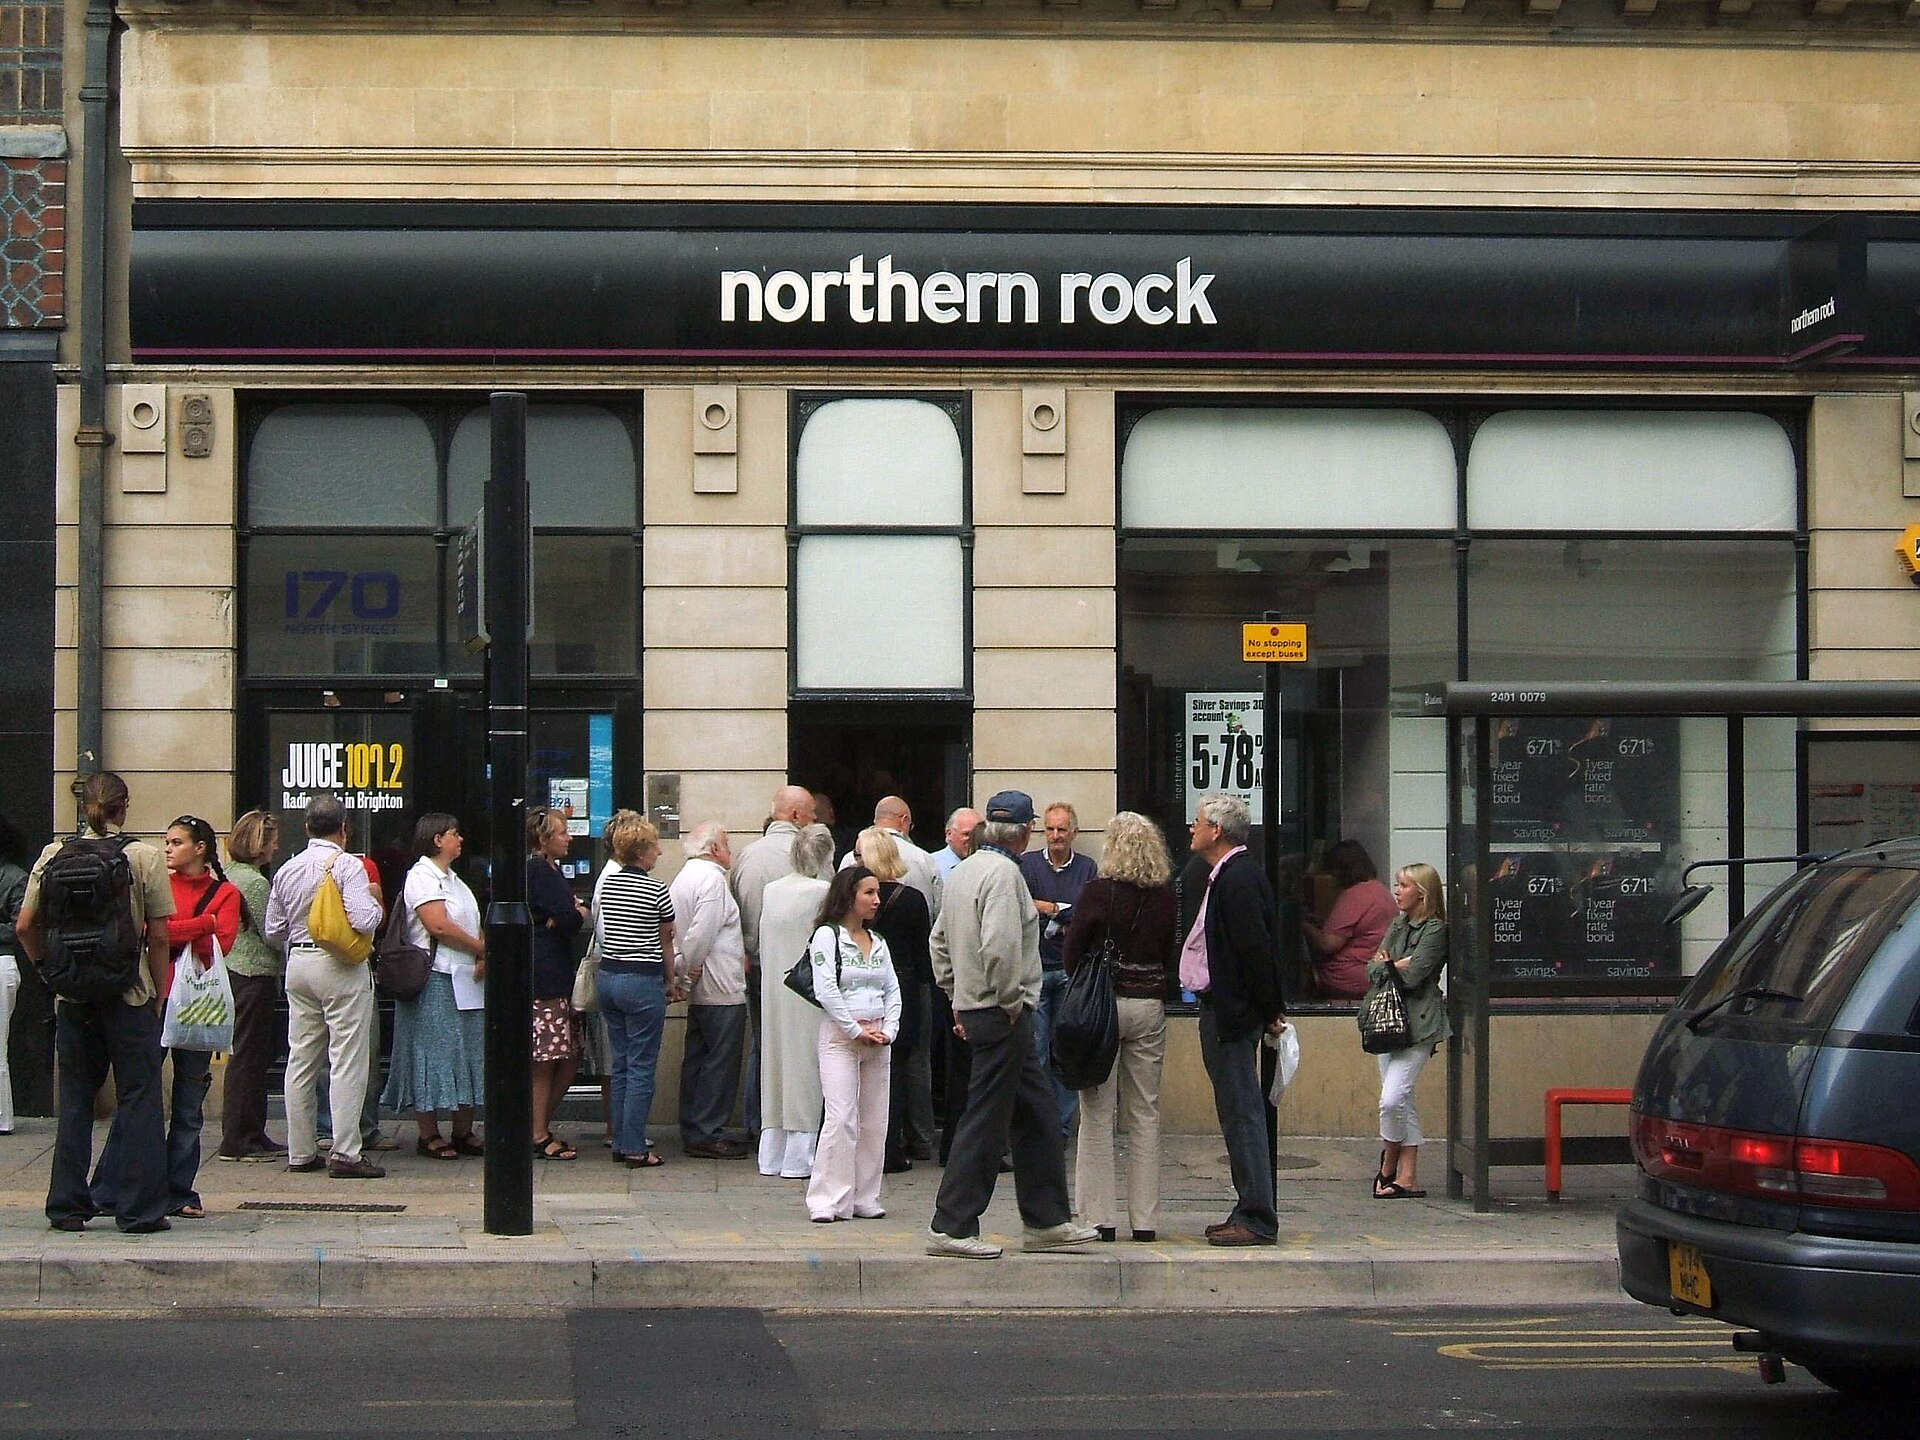
\includegraphics[height=0.40\textheight]{ch15_northern_rock_2007.jpg}\\[1mm]
\imgcap{Deponenți la coadă în fața unei sucursale Northern Rock, septembrie 2007}
\imgcredit{https://commons.wikimedia.org/wiki/File:Northern_Rock_Queue.jpg}{Foto: Dominic Alves (2007); CC BY 2.0; Wikimedia Commons}
\end{column}
\end{columns}
\end{frame}

\begin{frame}{Too big to fail}
\itemsize{\small}
\begin{itemize}
    \item \textbf{Too big to fail} (prea mare pentru a fi lăsată să falimenteze): o bancă al cărei faliment ar afecta economia atît de mult încît statul o salvează
    \begin{itemize}
        \item salvarea așteptată îi reduce costul de finanțare: o subvenție implicită
        \item hazard moral: banca își asumă mai mult risc, deoarece pierderile sînt împărțite cu contribuabilii
    \end{itemize}
    \item Răspunsul autorităților după 2008 \refGSIB
    \begin{itemize}
        \item G-SIB (global systemically important banks, bănci de importanță sistemică globală): o listă publicată anual, cu capital suplimentar pentru fiecare bancă
        \item planuri de rezoluție: o bancă aflată în dificultate trebuie lichidată fără banii contribuabililor
    \end{itemize}
    \item Măsurile din datele de piață (CoVaR, SRISK) permit ordonarea băncilor fără a aștepta un faliment
\end{itemize}
\end{frame}

\begin{frame}{Măsurile capitolului, pe scurt}
\itemsize{\small}
\begin{center}
\footnotesize
\begin{tabular}{>{\raggedright\arraybackslash}p{2.4cm}>{\raggedright\arraybackslash}p{5.6cm}>{\raggedright\arraybackslash}p{3.4cm}}
\toprule
\textbf{Măsura} & \textbf{Întrebarea} & \textbf{Instrumentul} \\
\midrule
corelația, dependența în cozi & se prăbușesc băncile și piețele împreună? & pseudo-observații, copula t \\
CoVaR, $\Delta$CoVaR & cu cît este mai rău sistemul cînd banca este în dificultate? & regresia cuantilică \\
MES & cît pierde banca în cele mai proaste zile ale pieței? & medie condiționată \\
SRISK & cît capital i-ar lipsi băncii într-o criză? & MES, efectul de levier \\
rețele & cine transmite șocuri și cui? & teste Granger, descompunerea varianței \\
\bottomrule
\end{tabular}
\end{center}
\begin{itemize}
    \item Toate măsurile folosesc doar prețurile de piață: sînt disponibile zilnic, pentru orice bancă listată
    \item Punctul lor slab: prețurile de piață pot fi liniștite în timp ce riscul se acumulează (2006--2007)
\end{itemize}
\end{frame}

\begin{frame}{Recapitulare: ce este riscul sistemic?}
\itemsize{\small}
\begin{itemize}
    \item Riscul sistemic: sistemul nu mai funcționează; este o proprietate a sistemului, nu a unui singur bilanț
    \item Canale: contagiunea directă, expunerile comune și vînzările forțate, retragerile masive și contagiunea informațională, toate amplificate de efectul de levier
    \item Măsurile privesc cozile comune: sistemul condiționat de bancă (CoVaR) sau banca condiționat de sistem (MES, SRISK)
\end{itemize}
\end{frame}


%=============================================================================
\section{Patru crize în date}
%=============================================================================

\begin{frame}{Datele capitolului}
\itemsize{\small}
\begin{center}
\scriptsize
\begin{tabular}{lll}
\toprule
\textbf{Grupul} & \textbf{Băncile} & \textbf{Indicele de piață} \\
\midrule
Bănci americane & JPMorgan Chase, Bank of America, Citigroup, Goldman Sachs, Morgan Stanley, Wells Fargo & S\&P 500 \\
Bănci europene & Deutsche Bank, BNP Paribas, Santander, ING, HSBC & Euro Stoxx 50 \\
Bănci românești & Banca Transilvania (TLV), BRD (din 2010) & BET \\
\bottomrule
\end{tabular}
\end{center}
\begin{itemize}
    \item Prețuri de închidere ajustate zilnice ale băncilor și închiderile indicilor, de la EODHD, ianuarie 2005 -- 18 septembrie 2026; VIX ca indicator de stres
    \item Prețurile se aliniază întîi pe zilele comune, apoi se calculează randamentele logaritmice zilnice în \%: $r_t = 100(\ln P_t - \ln P_{t-1})$
    \item Băncile BVB din 2010: înainte, multe zile nu au tranzacții; TLV fără 30--31 mai 2016 (o ajustare de preț aplicată cu o zi mai tîrziu, \sfmchlink{https://danpele.github.io/SFM/RO/Cursuri/capitol2_distributii_clasice_fapte_stilizate.pdf}{Capitolul 2})
    \item Portofoliul de bănci al unui grup: ponderi egale, reechilibrate zilnic
\end{itemize}
\end{frame}

\begin{frame}{Portofoliile de bănci din 2005}
\itemsize{\footnotesize}
\begin{center}
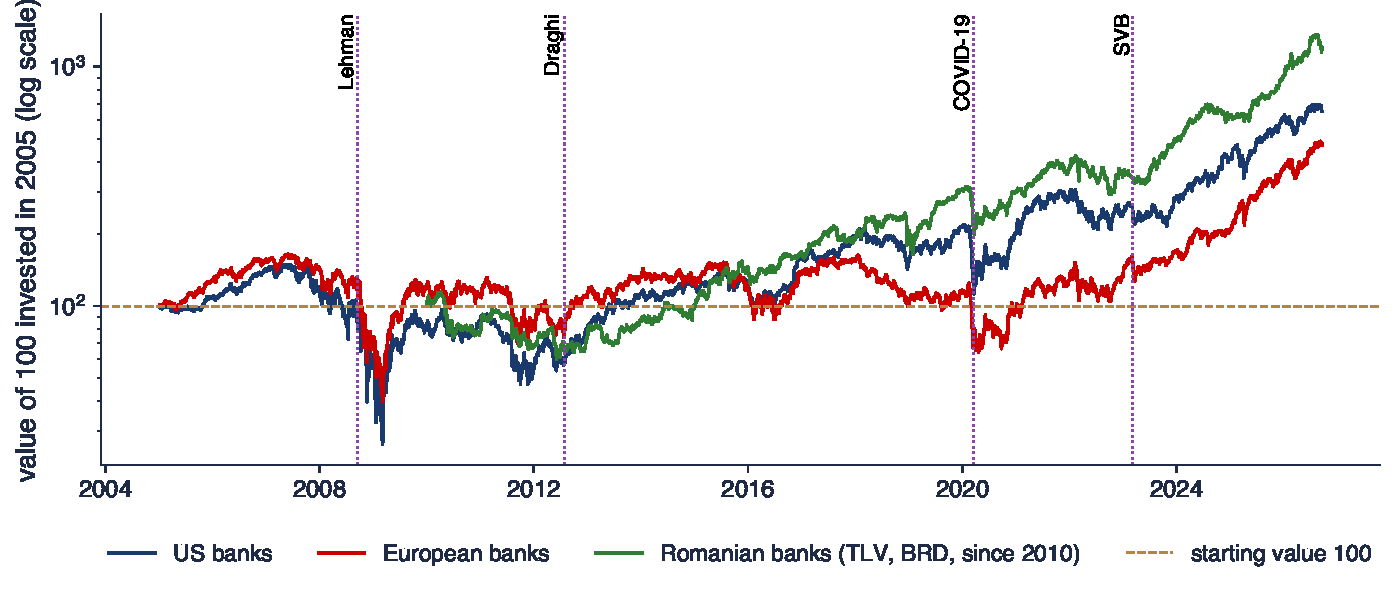
\includegraphics[width=0.97\textwidth,height=0.64\textheight,keepaspectratio]{sfm_ch15_bank_indices.pdf}
\end{center}
\vspace{-0.25cm}
\begin{itemize}
    \item Valoarea a 100 de unități investite în fiecare portofoliu cu ponderi egale (scară logaritmică); linii punctate: Lehman, discursul lui Draghi, COVID-19, falimentul SVB
    \item Drawdown maxim: băncile americane $-82\%$ (6 martie 2009), băncile europene $-76\%$ (9 martie 2009), băncile românești $-47\%$ (5 iunie 2012)
\end{itemize}
\sfmquantlet{Ch_15}{SFM_ch15_crises}
\end{frame}

\begin{frame}{Interpretarea portofoliilor de bănci}
\itemsize{\small}
\begin{itemize}
    \item 2008--2009: băncile americane și europene au pierdut aproximativ patru cincimi din valoare; minimul a venit în martie 2009, la șase luni după Lehman
    \begin{itemize}
        \item o criză sistemică este un proces care durează luni, nu o singură zi proastă
    \end{itemize}
    \item Băncile europene au rămas sub nivelul din 2005 în cea mai mare parte a perioadei: criza din zona euro și dobînzile scăzute
    \item Băncile românești: cea mai mare scădere a venit în criza din zona euro din 2011--2012 (băncile-mamă ale multor bănci din România sînt în zona euro)
    \item Martie 2020 și martie 2023: scăderi abrupte, dar scurte; băncile centrale și guvernele au reacționat în cîteva zile
\end{itemize}
\end{frame}

\begin{frame}{2008: Lehman Brothers}
\itemsize{\footnotesize}
\begin{columns}[T]
\begin{column}{0.58\textwidth}
\begin{itemize}
    \item 15 septembrie 2008: Lehman Brothers intră în faliment, cel mai mare faliment din istoria SUA (active de peste 600 de miliarde USD)
    \begin{itemize}
        \item 16 septembrie: AIG, un asigurător care vînduse multor bănci protecție pentru datoriile ipotecare, este salvat de Rezerva Federală
        \item în aceeași zi, un fond monetar cu titluri Lehman scade sub un dolar pe unitate, iar investitorii își retrag banii din astfel de fonduri
    \end{itemize}
    \item Toate cele trei canale simultan
    \begin{itemize}
        \item expuneri directe (derivate cu Lehman), expuneri comune (credite ipotecare), retragerea finanțării pe termen scurt
    \end{itemize}
    \item De la sfîrșitul lui august pînă la minimul din noiembrie: băncile americane $-59\%$, cele europene $-54\%$, S\&P 500 $-41\%$
\end{itemize}
\end{column}
\begin{column}{0.38\textwidth}
\centering
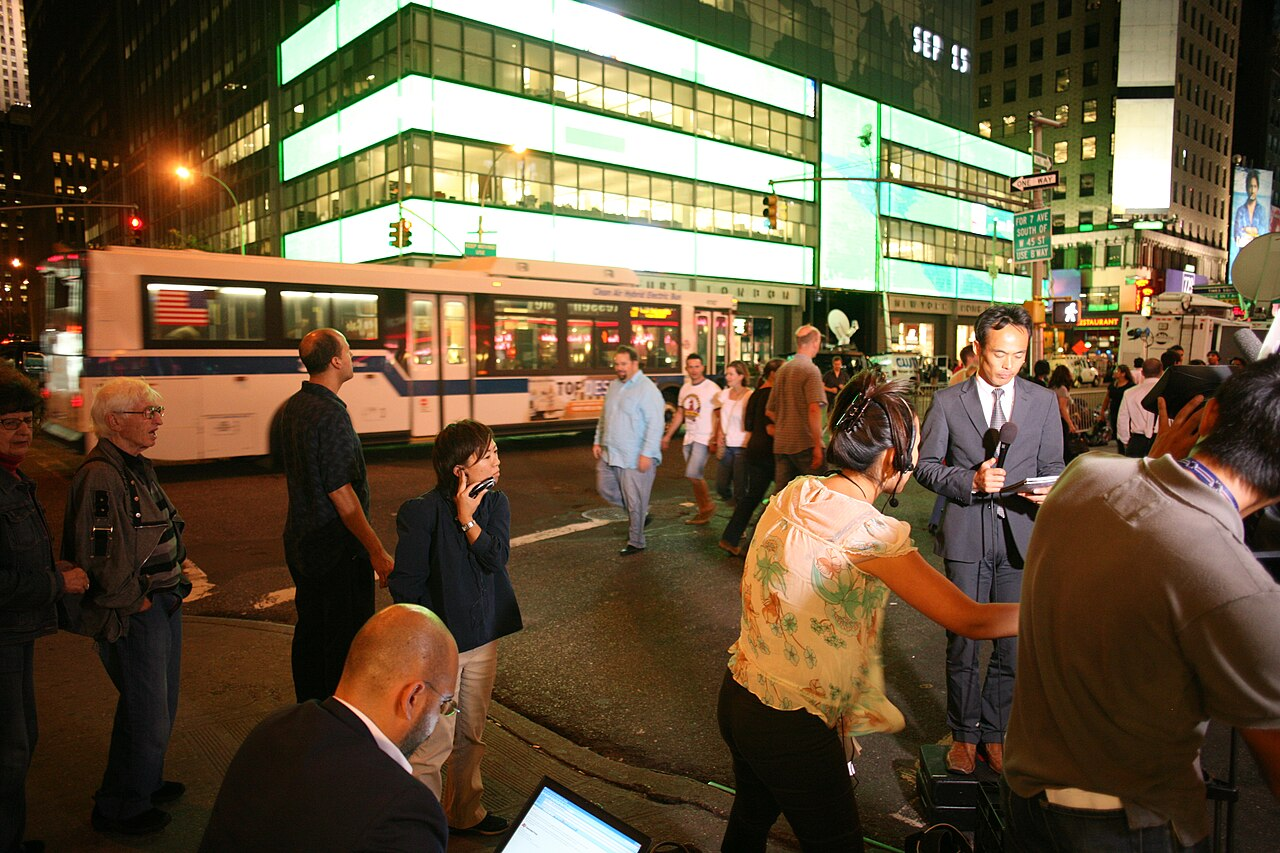
\includegraphics[height=0.40\textheight]{ch0_lehman_2008.jpg}\\[1mm]
\imgcap{Sediul Lehman Brothers, New York, 15 septembrie 2008}
\imgcredit{https://commons.wikimedia.org/wiki/File:Lehman_Brothers-NYC-20080915.jpg}{Foto: Robert Scoble (2008); CC BY 2.0; Wikimedia Commons}
\end{column}
\end{columns}
\end{frame}

\begin{frame}{2010--2012: criza din zona euro}
\itemsize{\footnotesize}
\begin{columns}[T]
\begin{column}{0.60\textwidth}
\begin{itemize}
    \item Grecia (2010), apoi Irlanda, Portugalia, Spania și Italia: îndoieli privind datoria publică
    \begin{itemize}
        \item \textbf{bucla bănci--stat}: băncile dețin obligațiunile propriului stat, iar statul garantează băncile
        \item o scădere a prețului obligațiunilor slăbește băncile; salvarea băncilor slăbește statul
    \end{itemize}
    \item 26 iulie 2012: Mario Draghi, președintele ECB (European Central Bank, Banca Centrală Europeană): „Banca Centrală Europeană este pregătită să facă tot ce este necesar pentru a păstra moneda euro” \refDraghi
    \begin{itemize}
        \item o promisiune, nu o cumpărare, a oprit spirala: rolul așteptărilor
    \end{itemize}
    \item Iulie 2011 -- septembrie 2012, punctul cel mai slab: băncile europene $-41\%$, cele americane $-37\%$, cele românești $-34\%$
\end{itemize}
\end{column}
\begin{column}{0.36\textwidth}
\centering

\includegraphics[height=0.30\textheight]{ch15_ecb_frankfurt_2015.jpg}\\[1mm]
\imgcap{Clădirea ECB din Frankfurt am Main}
\imgcredit{https://commons.wikimedia.org/wiki/File:Seat_of_the_European_Central_Bank_and_Frankfurt_Skyline_at_dawn_20150422_1.jpg}{Foto: D\-XR (2015); CC BY-SA 4.0; Wikimedia Commons}
\end{column}
\end{columns}
\end{frame}

\begin{frame}{Martie 2020: goana după lichiditate}
\itemsize{\footnotesize}
\begin{columns}[T]
\begin{column}{0.58\textwidth}
\begin{itemize}
    \item Restricțiile COVID-19: toată lumea a vrut lichiditate în același timp; s-au vîndut chiar și obligațiunile de stat
    \begin{itemize}
        \item stresul a pornit din afara băncilor: fonduri, firme, piața obligațiunilor
        \item băncile erau mai bine capitalizate decît în 2008 (Basel III) și au devenit parte a soluției (liniile de credit)
    \end{itemize}
    \item Răspuns rapid al autorităților: băncile centrale au cumpărat active și au împrumutat dolari altor bănci centrale
    \begin{itemize}
        \item minimul pe 23 martie 2020: băncile americane $-48\%$, cele europene $-48\%$, cele românești $-35\%$, S\&P 500 $-34\%$
    \end{itemize}
\end{itemize}
\end{column}
\begin{column}{0.38\textwidth}
\centering
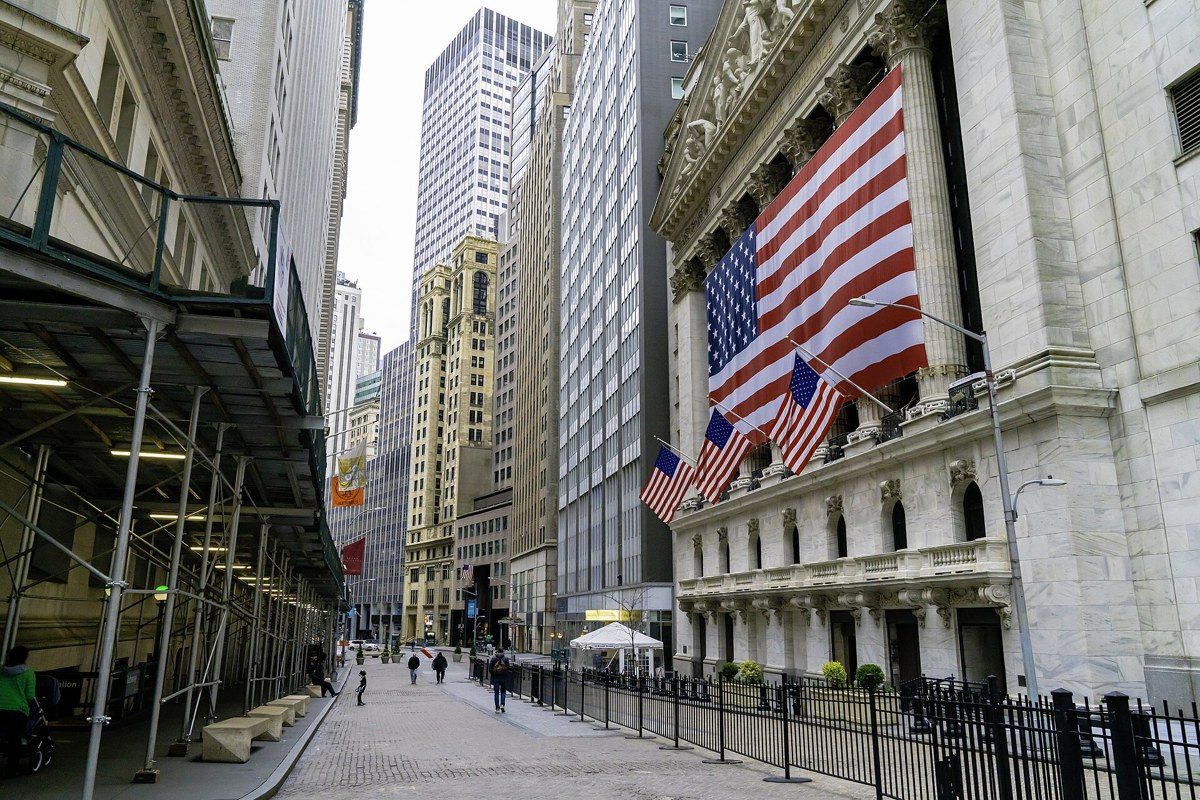
\includegraphics[height=0.38\textheight]{ch0_fidi_march_2020.jpg}\\[1mm]
\imgcap{Districtul financiar din New York, 25 martie 2020}
\imgcredit{https://commons.wikimedia.org/wiki/File:Subdued_FiDi_(50063555551).jpg}{Foto: Billie Grace Ward (2020); CC BY 2.0; Wikimedia Commons}
\end{column}
\end{columns}
\end{frame}

\begin{frame}{Martie 2023: SVB}
\itemsize{\footnotesize}
\begin{columns}[T]
\begin{column}{0.58\textwidth}
\begin{itemize}
    \item SVB (Silicon Valley Bank): depozite ale firmelor de tehnologie, majoritatea peste plafonul garantat, investite în obligațiuni pe termen lung
    \begin{itemize}
        \item creșterea dobînzilor din 2022 a produs pierderi mari nerealizate pe obligațiuni
        \item 9 martie 2023: deponenții au încercat să retragă aproximativ 42 de miliarde USD într-o singură zi; 10 martie: banca este închisă \refFed; \refFDIC
    \end{itemize}
    \item O retragere masivă în epoca aplicațiilor bancare: mai rapidă decît oricare alta înainte
    \begin{itemize}
        \item o bancă de mărime medie a devenit sistemică prin contagiune informațională: alte bănci regionale au scăzut în zilele următoare
    \end{itemize}
\end{itemize}
\end{column}
\begin{column}{0.38\textwidth}
\centering

\includegraphics[height=0.38\textheight]{ch15_svb_hq_2023.jpg}\\[1mm]
\imgcap{Sediul Silicon Valley Bank, Santa Clara, 13 martie 2023}
\imgcredit{https://commons.wikimedia.org/wiki/File:3003_West_Tasman_Drive_entrance_2,_Santa_Clara,_California.jpg}{Foto: Minh Nguyen (2023); CC BY-SA 4.0; Wikimedia Commons}
\end{column}
\end{columns}
\end{frame}

\begin{frame}{Martie 2023: Credit Suisse}
\itemsize{\footnotesize}
\begin{columns}[T]
\begin{column}{0.60\textwidth}
\begin{itemize}
    \item Credit Suisse: o bancă G-SIB care pierdea de ani de zile clienți și bani (scandaluri, pierderi cu clienți de tip hedge fund)
    \begin{itemize}
        \item după SVB, investitorii și deponenții au plecat repede
    \end{itemize}
    \item 19 martie 2023: preluarea de către UBS, aprobată de autoritatea elvețiană de supraveghere FINMA \refFINMA
    \begin{itemize}
        \item obligațiunile AT1 (additional tier 1, capital suplimentar de nivel 1) de aproximativ 16 miliarde CHF au fost anulate
        \item o salvare prin fuziune, nu o rezoluție: problema too big to fail nu dispăruse
    \end{itemize}
    \item De la sfîrșitul lui februarie pînă la minim: băncile europene $-21\%$, cele americane $-16\%$, cele românești $-7\%$
\end{itemize}
\end{column}
\begin{column}{0.36\textwidth}
\centering
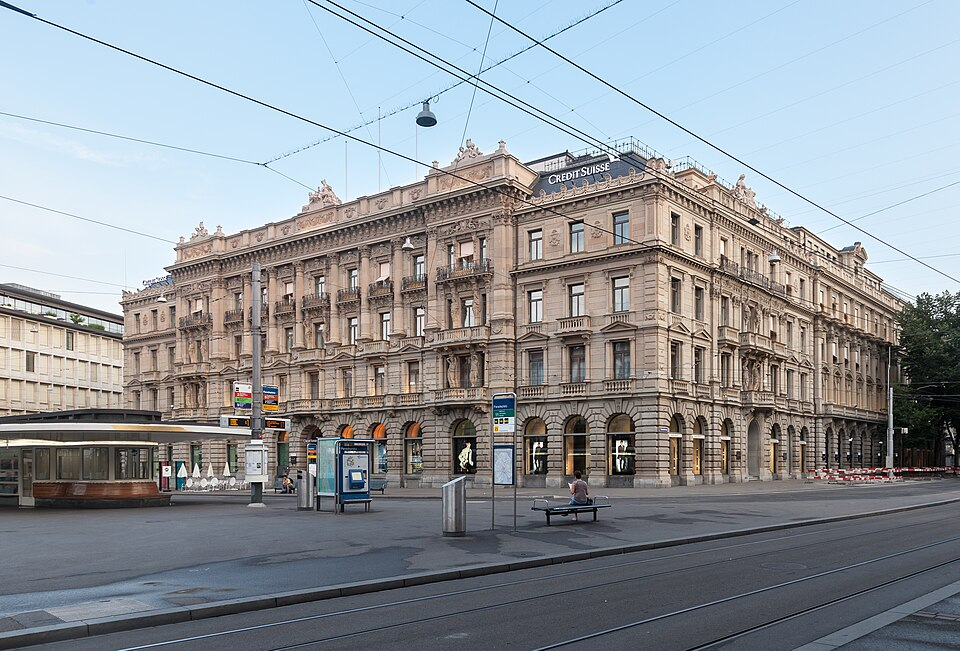
\includegraphics[height=0.28\textheight]{ch15_credit_suisse_zurich_2013.jpg}\\[1mm]
\imgcap{Sediul Credit Suisse din Paradeplatz, Zürich}
\imgcredit{https://commons.wikimedia.org/wiki/File:Credit_Suisse_Z\%C3\%BCrich.jpg}{Foto: Thomas Wolf, www.foto-tw.de (2013); CC BY-SA 3.0 DE; Wikimedia Commons}
\end{column}
\end{columns}
\end{frame}

\begin{frame}{Patru episoade comparate}
\itemsize{\footnotesize}
\begin{center}
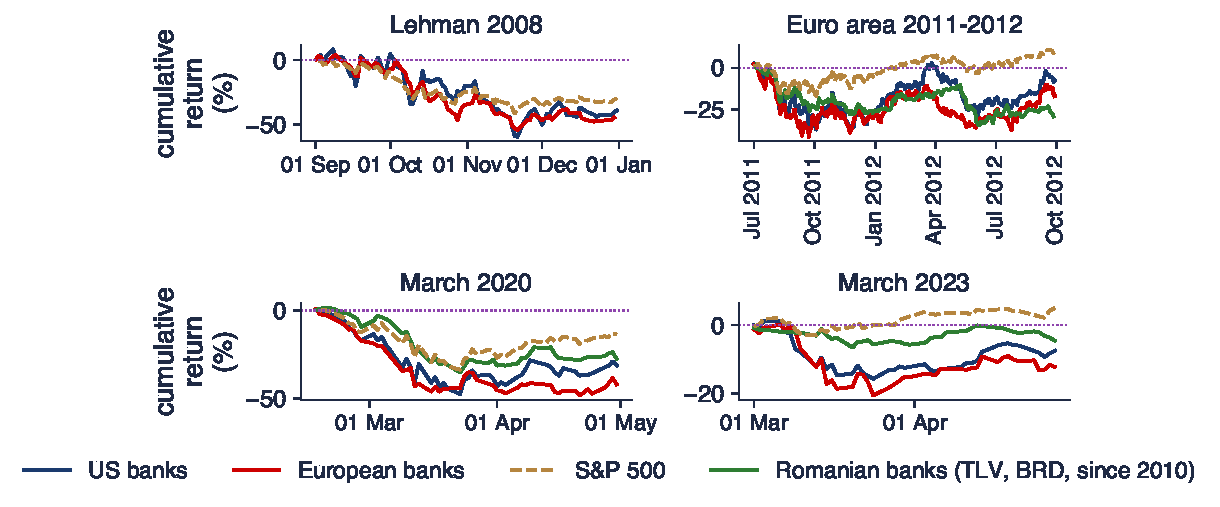
\includegraphics[width=0.97\textwidth,height=0.64\textheight,keepaspectratio]{sfm_ch15_episodes.pdf}
\end{center}
\vspace{-0.25cm}
\begin{itemize}
    \item Randamentul cumulat de la începutul fiecărei ferestre; băncile românești intră în date în 2010
    \item Interpretare: în 2008 și 2011--2012 băncile au scăzut mult mai mult decît S\&P 500 (băncile erau problema); în 2020 au scăzut odată cu piața; în 2023 au scăzut în timp ce piața creștea
\end{itemize}
\sfmquantlet{Ch_15}{SFM_ch15_crises}
\end{frame}

\begin{frame}{Recapitulare: patru crize}
\itemsize{\small}
\begin{itemize}
    \item 2008: contagiune prin derivate, expuneri comune la creditele ipotecare și retragerea finanțării pe termen scurt
    \item 2011--2012: bucla bănci--stat; oprită de o promisiune a băncii centrale
    \item 2020: un șoc din exterior, întîmpinat de bănci mai bine capitalizate; 2023: retrageri digitale și contagiune informațională
\end{itemize}
\end{frame}


%=============================================================================
\section{Corelația și dependența în cozi în crize}
%=============================================================================

\begin{frame}{Corelația dintre bănci crește în crize}
\itemsize{\footnotesize}
\begin{center}
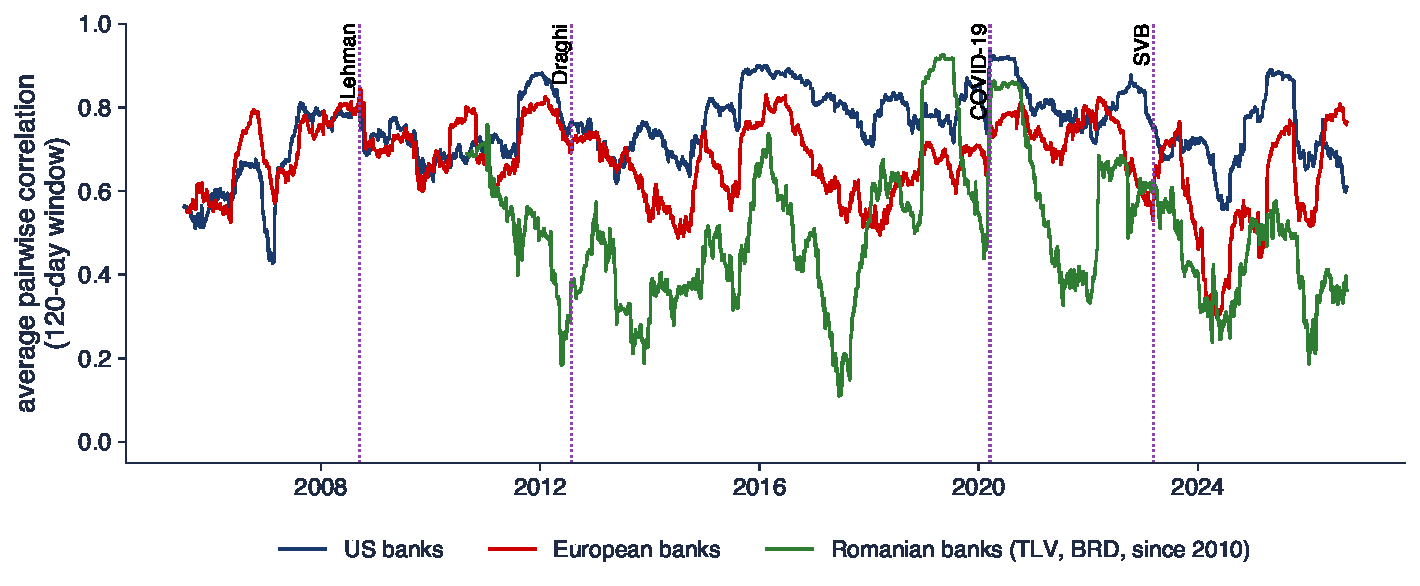
\includegraphics[width=0.97\textwidth,height=0.62\textheight,keepaspectratio]{sfm_ch15_rolling_corr.pdf}
\end{center}
\vspace{-0.25cm}
\begin{itemize}
    \item Media corelațiilor dintre perechile de bănci, pe randamente zilnice, în fiecare grup, pe ferestre de 120 de zile
    \item Băncile americane: $0{,}59$ înainte de criză (iulie 2005 -- iunie 2007), pînă la $0{,}94$ (16 martie 2020); TLV și BRD: $0{,}31$ în 2017, $0{,}85$ în aprilie--iunie 2020
\end{itemize}
\sfmquantlet{Ch_15}{SFM_ch15_dependence}
\end{frame}

\begin{frame}{Interpretarea corelațiilor: cînd diversificarea nu mai funcționează}
\itemsize{\small}
\begin{itemize}
    \item În crize, băncile se mișcă împreună: un portofoliu de mai multe bănci este aproape o singură bancă
    \begin{itemize}
        \item factorul comun (piața, stresul de finanțare) domină știrile specifice fiecărei bănci
    \end{itemize}
    \item Cele două bănci românești: corelație mică în anii liniștiți, foarte mare în 2020
    \begin{itemize}
        \item în anii liniștiți, acțiunile BVB sînt determinate de propriile știri și de lichiditatea redusă; într-o criză, de șocul comun
    \end{itemize}
    \item Atenție: o corelație pe 120 de zile este zgomotoasă, iar o creștere a corelației nu dovedește contagiunea (slide-ul următor)
\end{itemize}
\end{frame}

\begin{frame}{Contagiune sau interdependență? Forbes și Rigobon}
\itemsize{\footnotesize}
\begin{itemize}
    \item Dacă $y = \beta x + e$ cu $\beta$ fix, corelația dintre $x$ și $y$ crește \textbf{automat} cînd crește varianța lui $x$ \refFR
    \begin{itemize}
        \item o corelație mai mare într-o criză poate fi aceeași legătură, văzută într-o perioadă mai volatilă: \textbf{interdependență}
        \item \textbf{contagiune}: legătura însăși devine mai puternică
    \end{itemize}
    \item Corelația corectată: $\rho^* = \rho / \sqrt{1 + \delta(1 - \rho^2)}$, cu $\delta = \sigma^2_{\text{criză}} / \sigma^2_{\text{calm}} - 1$ pentru piața-sursă
    \begin{itemize}
        \item Portofoliul băncilor americane (sursa) și cel al băncilor europene: perioada calmă ianuarie 2005 -- iunie 2007 ($n = 506$), criza 15 septembrie -- 31 decembrie 2008 ($n = 72$)
        \item $\rho_{\text{calm}} = 0{,}40$, $\rho_{\text{criză}} = 0{,}60$; varianța $0{,}89$ $\to$ $75{,}4$, deci $\delta = 83{,}7$
        \item $\rho^* = 0{,}60/\sqrt{1 + 83{,}7 \times 0{,}64} = 0{,}60/\sqrt{54{,}4} = 0{,}08$
    \end{itemize}
    \item Interpretare: după corecție, corelația nu mai crește: datele sînt compatibile cu interdependența, nu cu o legătură mai puternică
\end{itemize}
\end{frame}

\begin{frame}{Dependența în cozi (\sfmchlinkt{https://danpele.github.io/SFM/RO/Cursuri/capitol10_var_es_backtesting.pdf}{Capitolul 10})}
\itemsize{\small}
\begin{itemize}
    \item Pseudo-observațiile $U = $ rang$/(n + 1)$; \textbf{dependența în coada inferioară} la nivelul $q$: $\lambda(q) = P(U_1 \le q \mid U_2 \le q)$
    \begin{itemize}
        \item la independență, $\lambda(q) = q$; limita $\lambda_L = \lim_{q \to 0}\lambda(q)$ este coeficientul de dependență în coadă
    \end{itemize}
    \item Copula t (\sfmchlink{https://danpele.github.io/SFM/RO/Cursuri/capitol10_var_es_backtesting.pdf}{Capitolul 10}) are $\lambda_L = 2t_{\nu+1}(-\sqrt{(\nu + 1)(1 - \rho)/(1 + \rho)}) > 0$ \refDM; copula Gaussiană are $\lambda_L = 0$
    \begin{itemize}
        \item $\rho = \sin(\pi\tau/2)$ din $\tau$ al lui Kendall, $\nu$ prin verosimilitate maximă
    \end{itemize}
    \item Pentru riscul sistemic: dependența în cozi măsoară cît de des sînt o bancă și piața \textbf{împreună} în cele mai proaste zile ale lor
\end{itemize}
\end{frame}

\begin{frame}{Dependența în cozi dintre bănci și piețe}
\itemsize{\footnotesize}
\begin{center}
\scriptsize
\begin{tabular}{lrrrrrr}
\toprule
\textbf{Perechea} & $n$ & corel. & $\lambda(5\%)$ & $\lambda(1\%)$ & $\hat\nu$ & $\lambda_L$ (t) \\
\midrule
bănci americane, S\&P 500 & 5\,229 & $0{,}79$ & $0{,}64$ & $0{,}63$ & $3{,}2$ & $0{,}49$ \\
bănci europene, Euro Stoxx 50 & 5\,212 & $0{,}86$ & $0{,}72$ & $0{,}67$ & $3{,}1$ & $0{,}59$ \\
bănci românești, BET & 3\,414 & $0{,}86$ & $0{,}65$ & $0{,}62$ & $4{,}3$ & $0{,}53$ \\
bănci europene, bănci americane & 4\,895 & $0{,}59$ & $0{,}43$ & $0{,}50$ & $3{,}0$ & $0{,}36$ \\
\bottomrule
\end{tabular}
\end{center}
\begin{itemize}
    \item $\lambda(q)$: empirică; $\hat\nu$ și $\lambda_L$: copula t; la independență, $\lambda(5\%) = 0{,}05$ și $\lambda(1\%) = 0{,}01$
    \item Interpretare: în peste jumătate dintre cele mai proaste zile ale pieței, și băncile sînt în cele mai proaste zile ale lor; $\hat\nu$ mic (circa 3--4) înseamnă prăbușiri simultane puternice, pe care o copulă Gaussiană nu le surprinde deloc
    \item $\lambda(1\%)$ se sprijină pe cîteva zeci de zile: o estimare imprecisă
\end{itemize}\sfmquantlet{Ch_15}{SFM_ch15_dependence}
\end{frame}

\begin{frame}{Zile proaste comune}
\itemsize{\footnotesize}
\begin{center}
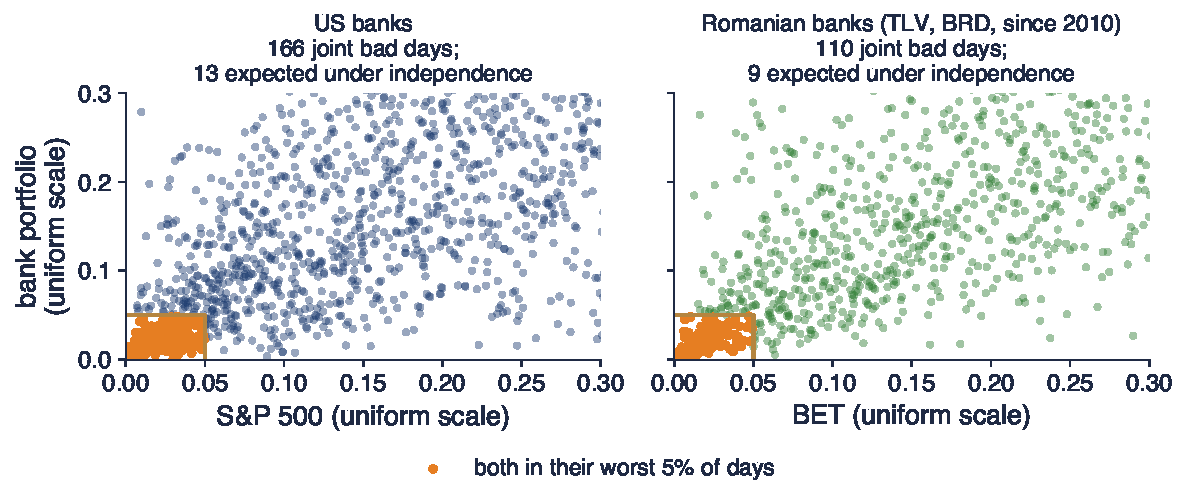
\includegraphics[width=0.97\textwidth,height=0.60\textheight,keepaspectratio]{sfm_ch15_tail_scatter.pdf}
\end{center}
\vspace{-0.25cm}
\begin{itemize}
    \item Colțul din stînga jos al pseudo-observațiilor; portocaliu: atît portofoliul de bănci, cît și indicele sînt în cele mai proaste 5\% dintre zile
    \item SUA: 166 de zile proaste comune, față de 13 la independență (de circa 13 ori mai multe); România: 110, față de 9
\end{itemize}
\sfmquantlet{Ch_15}{SFM_ch15_dependence}
\end{frame}

\begin{frame}{Recapitulare: corelația și dependența în cozi}
\itemsize{\small}
\begin{itemize}
    \item Corelațiile dintre bănci cresc în crize; diversificarea între bănci nu funcționează tocmai cînd este nevoie de ea
    \item O creștere a corelației nu este o dovadă de contagiune: corectați pentru creșterea volatilității (Forbes--Rigobon)
    \item Dependența în cozi (copula t, $\nu$ în jur de 3--4) arată prăbușiri simultane puternice ale băncilor și piețelor
\end{itemize}
\end{frame}


%=============================================================================
\section{CoVaR și Delta-CoVaR}
%=============================================================================

\begin{frame}{De la VaR la CoVaR}
\itemsize{\small}
\begin{itemize}
    \item $X^i$: randamentul instituției $i$; $X^{sys}$: randamentul sistemului; nivelul $\alpha$ = probabilitatea cozii (\sfmchlink{https://danpele.github.io/SFM/RO/Cursuri/capitol10_var_es_backtesting.pdf}{Capitolul 10})
    \begin{itemize}
        \item $\mathrm{VaR}^i_\alpha = -q_\alpha(X^i)$: pierderea lui $i$ depășită cu probabilitatea $\alpha$
    \end{itemize}
    \item \textbf{CoVaR} (VaR-ul condiționat al sistemului) \refAB: $\mathrm{CoVaR}^{sys|i}_\alpha = -q_\alpha\big(X^{sys} \mid X^i = q_\alpha(X^i)\big)$
    \begin{itemize}
        \item VaR 1\% al sistemului într-o zi în care instituția $i$ se află la propriul VaR 1\%: „CoVaR 1\%”
    \end{itemize}
    \item \textbf{$\Delta$CoVaR}: $\Delta\mathrm{CoVaR}^{sys|i}_\alpha = \mathrm{CoVaR}^{sys|X^i = q_\alpha}_\alpha - \mathrm{CoVaR}^{sys|X^i = q_{50\%}}_\alpha$
    \begin{itemize}
        \item cu cît crește VaR-ul sistemului cînd $i$ trece de la o zi obișnuită (mediana sa) la o zi de criză: \textbf{contribuția} lui $i$ la riscul sistemic
    \end{itemize}
\end{itemize}
\end{frame}

\begin{frame}{Regresia cuantilică (\sfmchlinkt{https://danpele.github.io/SFM/RO/Cursuri/capitol13_invatare_automata.pdf}{Capitolul 13})}
\itemsize{\small}
\begin{itemize}
    \item Regresia cuantilică liniară \refKB: $q_\alpha(Y \mid X = x) = a_\alpha + b_\alpha x$
    \begin{itemize}
        \item estimată prin minimizarea $\sum_t \rho_\alpha(y_t - a - bx_t)$, cu funcția de pierdere $\rho_\alpha(u) = u(\alpha - \mathbf{1}\{u < 0\})$
        \item pentru $\alpha = 1\%$, un reziduu sub dreaptă costă de 99 de ori mai mult decît unul deasupra ei: dreapta trece sub 99\% dintre puncte
    \end{itemize}
    \item Aceeași idee ca VaR 1\% prin regresie cuantilică din \sfmchlink{https://danpele.github.io/SFM/RO/Cursuri/capitol13_invatare_automata.pdf}{Capitolul 13}, acum cu o altă instituție ca variabilă explicativă
    \begin{itemize}
        \item panta $b_\alpha$ poate diferi de panta OLS: coada poate reacționa mai puternic decît centrul
    \end{itemize}
    \item $a_\alpha$ este termenul liber al regresiei, iar $b_\alpha$ este panta
\end{itemize}
\end{frame}

\begin{frame}{Estimarea CoVaR în trei pași}
\itemsize{\small}
\begin{itemize}
    \item \textbf{Pasul 1}: regresia cuantilică a sistemului pe instituție, la nivelul $\alpha$: $X^{sys}_t = a + bX^i_t + \varepsilon_t$ \refAB
    \begin{itemize}
        \item cuantila de ordin $\alpha$ a erorii este zero prin construcție
    \end{itemize}
    \item \textbf{Pasul 2}: cuantilele empirice ale instituției: $\hat q_\alpha(X^i)$ (dificultate) și $\hat q_{50\%}(X^i)$ (mediana)
    \item \textbf{Pasul 3}: înlocuim
    \begin{itemize}
        \item $\mathrm{CoVaR}_\alpha = -(\hat a + \hat b\,\hat q_\alpha(X^i))$
        \item $\Delta\mathrm{CoVaR}_\alpha = \hat b\,\big(\hat q_{50\%}(X^i) - \hat q_\alpha(X^i)\big)$: contează doar panta și distanța dintre cele două cuantile
    \end{itemize}
    \item Aici sistemul este aproximat prin indicele bursier al regiunii (S\&P 500, Euro Stoxx 50, BET); Adrian și Brunnermeier folosesc portofoliul tuturor instituțiilor financiare
\end{itemize}
\end{frame}

\begin{frame}{Exemplu rezolvat: JPMorgan Chase și S\&P 500}
\itemsize{\small}
\begin{itemize}
    \item Randamente logaritmice zilnice, 2005--2026 ($n = 5\,229$); regresia cuantilică la 1\%: $\hat a = -2{,}35$, $\hat b = 0{,}39$
    \begin{itemize}
        \item JPM: $\hat q_{1\%} = -6{,}27\%$ (deci VaR 1\% al JPM $= 6{,}27\%$), mediana $\hat q_{50\%} = 0{,}07\%$
    \end{itemize}
    \item \textbf{CoVaR 1\%} $= -(-2{,}35 + 0{,}39 \times (-6{,}27)) = 2{,}35 + 2{,}44 = 4{,}79\%$
    \begin{itemize}
        \item CoVaR la mediana JPM: $2{,}32\%$
    \end{itemize}
    \item \textbf{$\Delta$CoVaR 1\%} $= 0{,}39 \times (0{,}07 - (-6{,}27)) = 0{,}39 \times 6{,}34 = 2{,}47\%$
    \begin{itemize}
        \item VaR 1\% necondiționat al S\&P 500 este $3{,}53\%$
    \end{itemize}
    \item Interpretare: cînd JPM este în dificultate, pierderea indicelui depășită cu probabilitatea 1\% este de 4{,}79\%, față de 2{,}32\% într-o zi obișnuită pentru JPM
\end{itemize}
\end{frame}

\begin{frame}{CoVaR într-un grafic}
\itemsize{\footnotesize}
\begin{center}
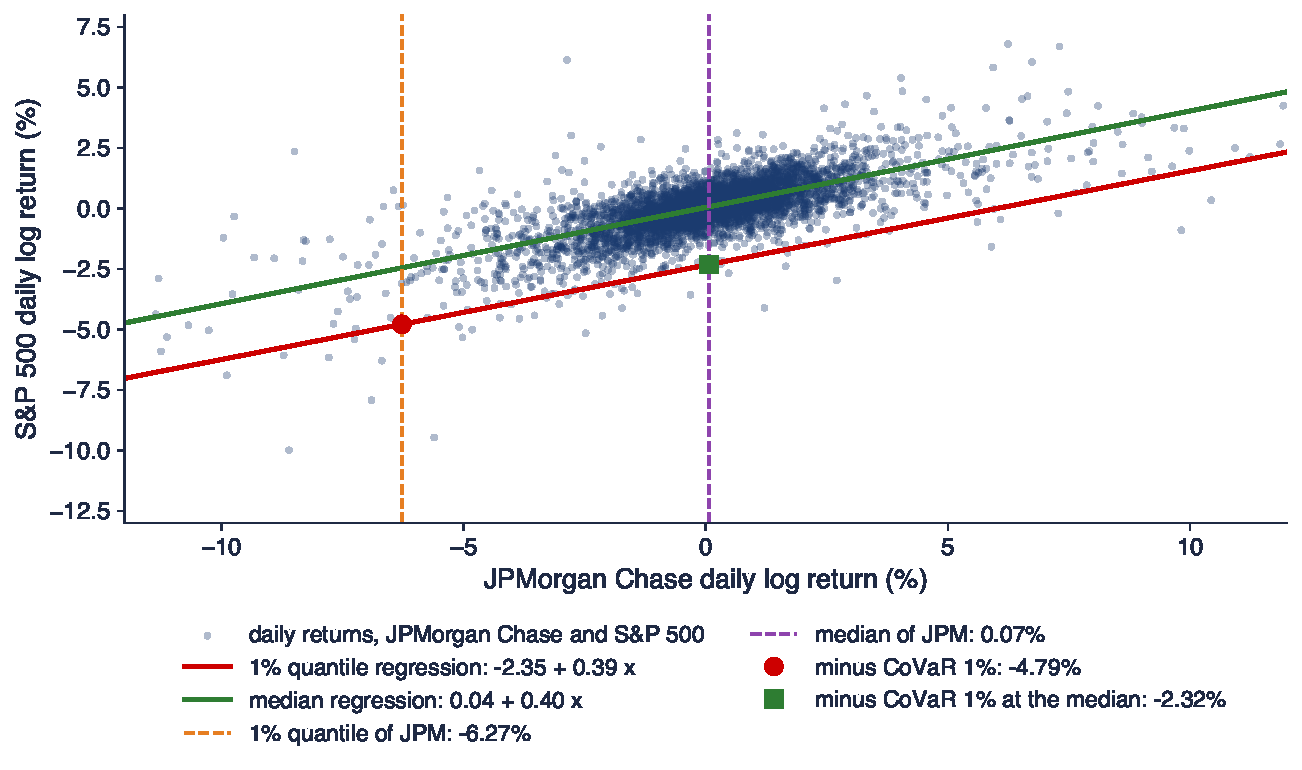
\includegraphics[width=0.97\textwidth,height=0.60\textheight,keepaspectratio]{sfm_ch15_covar_qr.pdf}
\end{center}
\vspace{-0.25cm}
\begin{itemize}
    \item Linia roșie: cuantila de 1\% a S\&P 500 condiționat de JPM; linia verde: mediana; linii întrerupte: cuantila de 1\% și mediana JPM
    \item $\Delta$CoVaR este distanța pe verticală dintre punctul roșu și pătratul verde de pe dreapta roșie: $2{,}47\%$
\end{itemize}
\sfmquantlet{Ch_15}{SFM_ch15_covar}
\end{frame}

\begin{frame}{$\Delta$CoVaR 1\% pentru 13 bănci}
\itemsize{\footnotesize}
\begin{center}
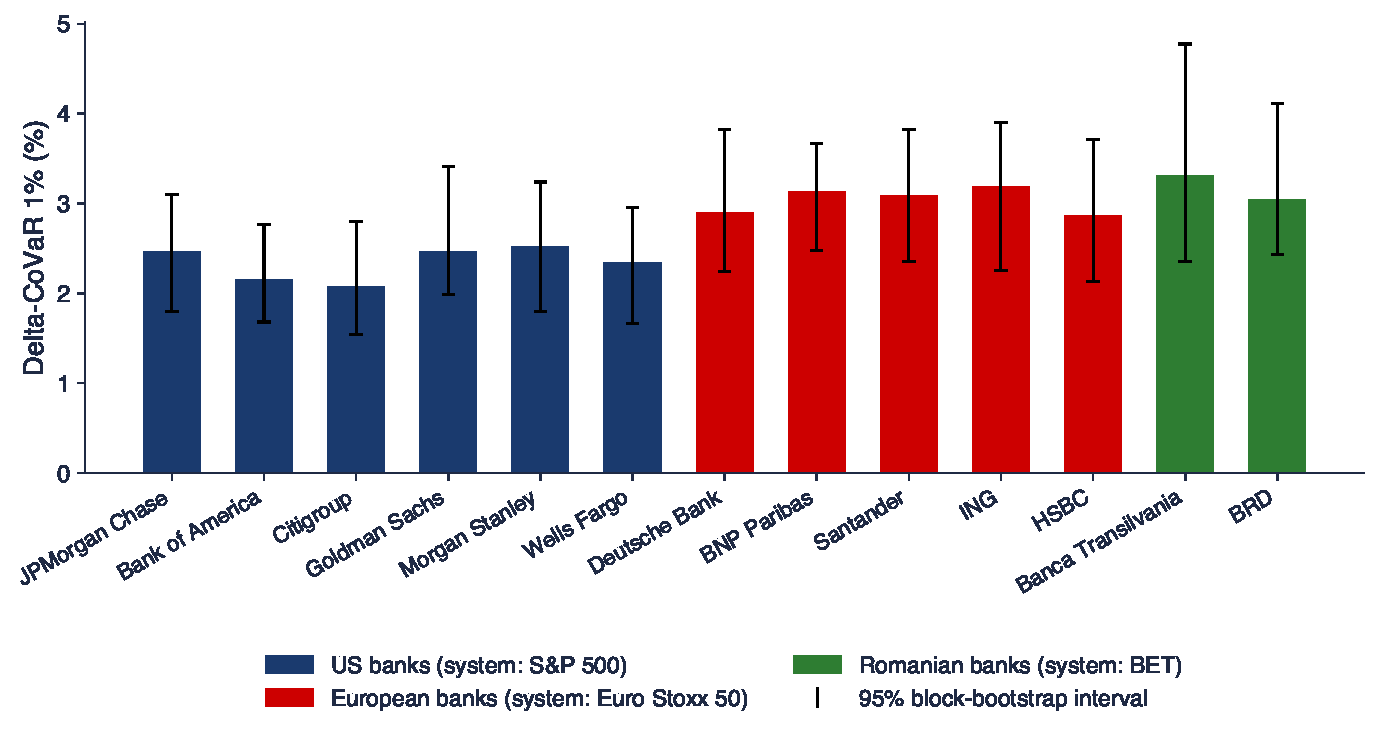
\includegraphics[width=0.97\textwidth,height=0.62\textheight,keepaspectratio]{sfm_ch15_dcovar.pdf}
\end{center}
\vspace{-0.25cm}
\begin{itemize}
    \item Sistemul: indicele regiunii; intervale de 95\% din bootstrap pe blocuri mobile (blocuri de 20 de zile, 200 de reeșantionări)
    \item Băncile americane: 2{,}1--2{,}5\%; băncile europene: 2{,}9--3{,}2\%; TLV $3{,}31\%$, BRD $3{,}05\%$; cel mai mare: Banca Transilvania
\end{itemize}
\sfmquantlet{Ch_15}{SFM_ch15_covar}
\end{frame}

\begin{frame}{Interpretarea $\Delta$CoVaR}
\itemsize{\small}
\begin{itemize}
    \item Intervalele se suprapun: în interiorul unei regiuni, datele nu pot ordona precis băncile
    \begin{itemize}
        \item orice ordonare după importanța sistemică trebuie însoțită de incertitudinea ei, ca orice estimare (bootstrap, \sfmchlink{https://danpele.github.io/SFM/RO/Cursuri/capitol2_distributii_clasice_fapte_stilizate.pdf}{Capitolul 2})
    \end{itemize}
    \item Băncile europene și cele românești au un $\Delta$CoVaR mai mare decît băncile americane
    \begin{itemize}
        \item băncile au o pondere mai mare în Euro Stoxx 50 și în BET decît în S\&P 500: indicele este mai aproape de un sistem bancar
        \item TLV și BRD sînt printre cele mai mari acțiuni din BET, deci BET le măsoară parțial chiar pe ele
    \end{itemize}
    \item Robustețe: ordinea la 5\% este apropiată de cea la 1\% (corelația Spearman $0{,}87$)
\end{itemize}
\end{frame}

\begin{frame}{Exemplu rezolvat: Banca Transilvania și BET}
\itemsize{\small}
\begin{itemize}
    \item TLV și BET, randamente logaritmice zilnice din 2010 ($n = 3\,414$); regresia cuantilică la 1\%: $\hat b = 0{,}61$
    \begin{itemize}
        \item TLV: $\hat q_{1\%} = -5{,}23\%$ (VaR 1\% al TLV), mediana $0{,}18\%$
    \end{itemize}
    \item $\Delta$CoVaR 1\% $= 0{,}61 \times (0{,}18 + 5{,}23) = 3{,}31\%$; CoVaR 1\% al BET $= 5{,}28\%$
    \begin{itemize}
        \item intervalul bootstrap pe blocuri de 95\% pentru $\Delta$CoVaR: [2{,}35; 4{,}78]
    \end{itemize}
    \item Interpretare: o zi de criză pentru TLV coboară cuantila de 1\% a BET cu aproximativ 3{,}31 puncte procentuale
    \begin{itemize}
        \item o parte este mecanică: TLV are una dintre cele mai mari ponderi în BET; un sistem mai curat ar fi BET fără TLV
    \end{itemize}
\end{itemize}
\end{frame}

\begin{frame}{VaR nu este $\Delta$CoVaR}
\itemsize{\footnotesize}
\begin{center}
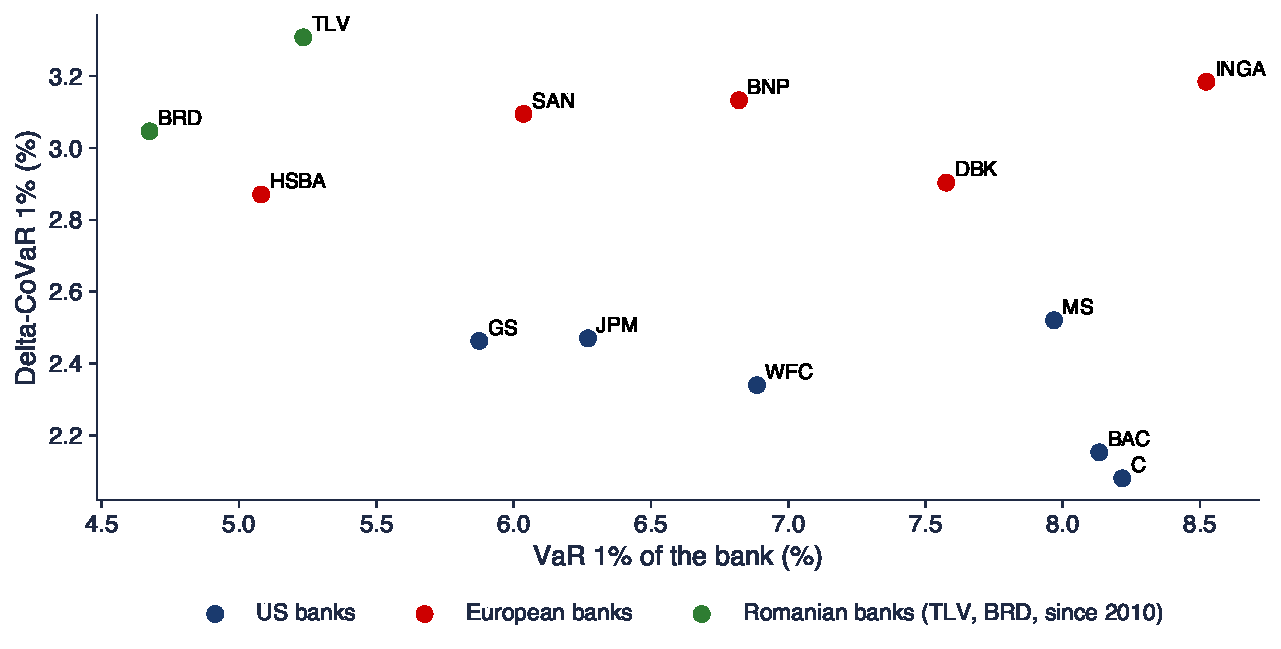
\includegraphics[width=0.97\textwidth,height=0.60\textheight,keepaspectratio]{sfm_ch15_var_vs_dcovar.pdf}
\end{center}
\vspace{-0.25cm}
\begin{itemize}
    \item Fiecare punct: o bancă, propriul VaR 1\% (orizontal) și $\Delta$CoVaR 1\% (vertical); corelația rangurilor Spearman $-0{,}31$
    \item Interpretare: Citigroup și Bank of America sînt printre primele trei după VaR 1\% și printre ultimele trei după $\Delta$CoVaR; reglementarea băncilor după propriul VaR scapă din vedere riscul sistemic \refAB
\end{itemize}
\sfmquantlet{Ch_15}{SFM_ch15_covar}
\end{frame}

\begin{frame}{$\Delta$CoVaR variabil în timp}
\itemsize{\small}
\begin{itemize}
    \item Adrian și Brunnermeier lasă cuantilele să depindă de \textbf{variabile de stare} $M_{t-1}$ decalate \refAB
    \begin{itemize}
        \item $X^i_t = c + \gamma^\top M_{t-1}$ la nivelurile $\alpha$ și 50\%: $\hat q_{\alpha,t}(X^i)$ și $\hat q_{50\%,t}(X^i)$
        \item $X^{sys}_t = a + bX^i_t + \delta^\top M_{t-1}$ la nivelul $\alpha$; apoi $\Delta\mathrm{CoVaR}_t = \hat b\,(\hat q_{50\%,t} - \hat q_{\alpha,t})$
    \end{itemize}
    \item Lucrarea folosește șapte variabile de stare (VIX, diferențe de lichiditate și de credit, dobînzi, randamentele pieței și ale sectorului imobiliar)
    \begin{itemize}
        \item aici, un set redus: nivelul VIX și randamentul indicelui din ziua precedentă
    \end{itemize}
    \item Panta $\hat b$ este fixă; variația în timp vine din distanța dintre cele două cuantile condiționate ale băncii
\end{itemize}
\end{frame}

\begin{frame}{$\Delta$CoVaR 1\% în timp}
\itemsize{\footnotesize}
\begin{center}
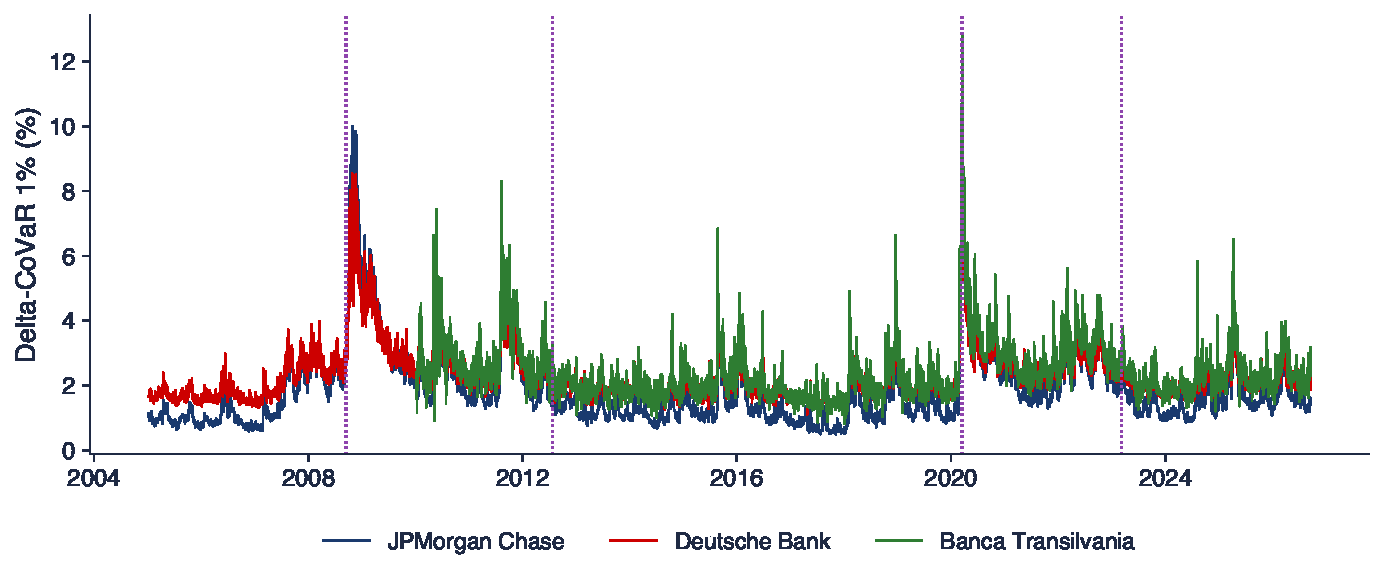
\includegraphics[width=0.97\textwidth,height=0.60\textheight,keepaspectratio]{sfm_ch15_dcovar_dynamic.pdf}
\end{center}
\vspace{-0.25cm}
\begin{itemize}
    \item JPMorgan Chase: media $1{,}86\%$, maximul $10{,}07\%$ (18 martie 2020); Deutsche Bank: maximul $9{,}08\%$ (13 martie 2020); Banca Transilvania: maximul $12{,}81\%$ (17 martie 2020)
    \item Interpretare: contribuția unei bănci la riscul sistemic nu este o constantă; crește brusc cînd crește VIX (2008, martie 2020) și este mică în anii liniștiți (JPM în 2017: $0{,}75\%$)
\end{itemize}
\sfmquantlet{Ch_15}{SFM_ch15_covar}
\end{frame}

\begin{frame}{Studiu de caz: Adrian și Brunnermeier (2016)}
\itemsize{\footnotesize}
\begin{columns}[T]
\begin{column}{0.56\textwidth}
\begin{itemize}
    \item \refAB: CoVaR pentru instituțiile financiare americane (bănci comerciale și de investiții, asigurători, brokeri), date săptămînale 1986--2010
    \begin{itemize}
        \item sistemul: portofoliul tuturor instituțiilor financiare; șapte variabile de stare
    \end{itemize}
    \item Rezultate
    \begin{itemize}
        \item în secțiunea transversală, VaR-ul unei instituții spune puțin despre $\Delta$CoVaR-ul ei
        \item $\Delta$CoVaR \textbf{prospectiv}: mărimea, efectul de levier și nepotrivirea scadențelor de acum doi ani prezic contribuția într-o criză
        \item o bază pentru capitalul anticiclic: cerințe mai mari cînd riscul se acumulează, nu cînd devine vizibil
    \end{itemize}
\end{itemize}
\end{column}
\begin{column}{0.42\textwidth}
\begin{columns}[T]
\begin{column}{0.48\textwidth}
\centering

\includegraphics[height=0.32\textheight]{ch15_adrian_2025.jpg}\\[1mm]
\imgcap{Tobias Adrian}
\imgcredit{https://commons.wikimedia.org/wiki/File:Tobias_Adrian_2025.jpg}{Foto: Chianoo Adrian (2025); CC BY 4.0; Wikimedia Commons}
\end{column}
\begin{column}{0.48\textwidth}
\centering

\includegraphics[height=0.32\textheight]{ch15_brunnermeier_2015.jpg}\\[1mm]
\imgcap{Markus Brunnermeier}
\imgcredit{https://commons.wikimedia.org/wiki/File:Markus_Konrad_Brunnermeier.jpg}{Foto: Iitkgpswapnil (2015); CC BY-SA 4.0; Wikimedia Commons}
\end{column}
\end{columns}
\end{column}
\end{columns}
\end{frame}

\begin{frame}{Recapitulare: CoVaR}
\itemsize{\small}
\begin{itemize}
    \item CoVaR 1\%: VaR 1\% al sistemului cînd instituția este la propriul VaR 1\%; $\Delta$CoVaR: creșterea de la o zi obișnuită la una de criză
    \item Estimat prin regresie cuantilică: $\Delta$CoVaR $= \hat b\,(\hat q_{50\%} - \hat q_\alpha)$
    \item VaR-ul propriu al unei bănci și contribuția ei sistemică ordonează diferit băncile; $\Delta$CoVaR variază puternic în timp
\end{itemize}
\end{frame}


%=============================================================================
\section{MES și SRISK}
%=============================================================================

\begin{frame}{Marginal expected shortfall (MES)}
\itemsize{\small}
\begin{itemize}
    \item \textbf{MES} \refAPPR: pierderea așteptată a instituției $i$ în zilele în care piața este în coada sa
    \begin{itemize}
        \item $\mathrm{MES}^i_\alpha = -E\big[X^i \mid X^m \le q_\alpha(X^m)\big]$; folosim cele mai proaste 5\% dintre zilele pieței: „MES 5\%”
        \item direcția este opusă celei din CoVaR: banca condiționat de piață, nu piața condiționat de bancă
    \end{itemize}
    \item De ce „marginal”: ES-ul pieței $= \sum_i w_i\,\mathrm{MES}^i$ cînd piața este un portofoliu cu ponderile $w_i$
    \begin{itemize}
        \item MES este contribuția lui $i$ la ES-ul sistemului (\sfmchlink{https://danpele.github.io/SFM/RO/Cursuri/capitol10_var_es_backtesting.pdf}{Capitolul 10})
    \end{itemize}
    \item Estimare: ordonăm zilele după randamentul pieței, luăm cele mai proaste $\lceil n\alpha \rceil$ zile, facem media randamentelor băncii în acele zile și schimbăm semnul
\end{itemize}
\end{frame}

\begin{frame}{Exemplu rezolvat: MES din zece zile}
\itemsize{\small}
\begin{center}
\footnotesize
\begin{tabular}{lrrrrrrrrrr}
\toprule
Ziua & 1 & 2 & 3 & 4 & 5 & 6 & 7 & 8 & 9 & 10 \\
\midrule
piața & $-4{,}0$ & $1{,}2$ & $-0{,}5$ & $2{,}1$ & $-6{,}0$ & $0{,}3$ & $-1{,}1$ & $0{,}8$ & $-2{,}2$ & $1{,}5$ \\
banca & $-6{,}5$ & $1{,}8$ & $-0{,}2$ & $2{,}9$ & $-9{,}0$ & $0{,}1$ & $-2{,}0$ & $1{,}1$ & $-3{,}1$ & $2{,}4$ \\
\bottomrule
\end{tabular}
\end{center}
\begin{itemize}
    \item Nivelul $\alpha = 20\%$: $\lceil 10 \times 0{,}2 \rceil = 2$ cele mai proaste zile ale pieței: ziua 5 ($-6{,}0$) și ziua 1 ($-4{,}0$)
    \begin{itemize}
        \item MES 20\% $= -(-9{,}0 - 6{,}5)/2 = 7{,}75\%$; ES 20\% al pieței $= -(-6{,}0 - 4{,}0)/2 = 5{,}00\%$
    \end{itemize}
    \item Interpretare: în zilele proaste ale pieței, această bancă pierde de aproximativ 1,5 ori mai mult decît piața: amplifică prăbușirile
    \item Observație: MES selectează zilele după randamentul pieței, nu după randamentul băncii
\end{itemize}
\end{frame}

\begin{frame}{MES 5\% pentru 13 bănci}
\itemsize{\footnotesize}
\begin{center}
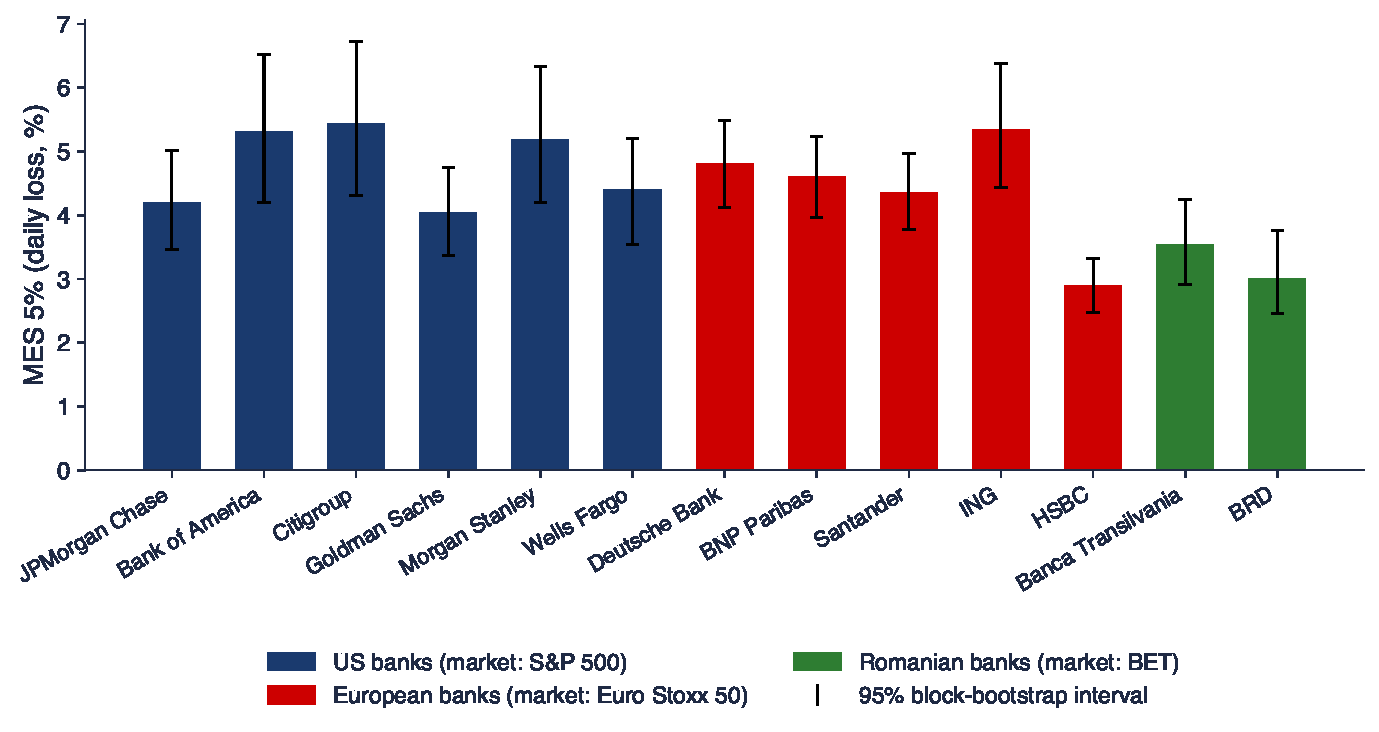
\includegraphics[width=0.97\textwidth,height=0.60\textheight,keepaspectratio]{sfm_ch15_mes.pdf}
\end{center}
\vspace{-0.25cm}
\begin{itemize}
    \item Pierderea zilnică medie a fiecărei bănci în cele mai proaste 5\% dintre zilele indicelui regiunii (SUA și Europa din 2005, România din 2010); intervale bootstrap pe blocuri de 95\%
    \item Cele mai mari: Citigroup ($5{,}44\%$) și ING ($5{,}35\%$); cel mai mic: HSBC ($2{,}90\%$); TLV $3{,}54\%$, BRD $3{,}00\%$
\end{itemize}
\sfmquantlet{Ch_15}{SFM_ch15_mes_srisk}
\end{frame}

\begin{frame}{Interpretarea MES și a $\Delta$CoVaR}
\itemsize{\small}
\begin{itemize}
    \item MES este apropiat de un beta al cozii: pierderea medie a pieței în cele mai proaste 5\% dintre zile, înmulțită cu sensibilitatea băncii
    \begin{itemize}
        \item Citigroup: beta OLS $1{,}66$, MES $5{,}44\%$; HSBC: beta $0{,}81$, MES $2{,}90\%$
    \end{itemize}
    \item MES și $\Delta$CoVaR ordonează diferit cele 13 bănci: corelația Spearman $-0{,}29$
    \begin{itemize}
        \item răspund la întrebări diferite: „cine suferă într-o prăbușire” față de „cine contribuie la prăbușire”
        \item o autoritate de reglementare ar trebui să privească mai multe măsuri, cu intervalele lor \refBCHP
    \end{itemize}
\end{itemize}
\end{frame}

\begin{frame}{Studiu de caz: a prezis MES pierderile din 2008?}
\itemsize{\footnotesize}
\begin{center}
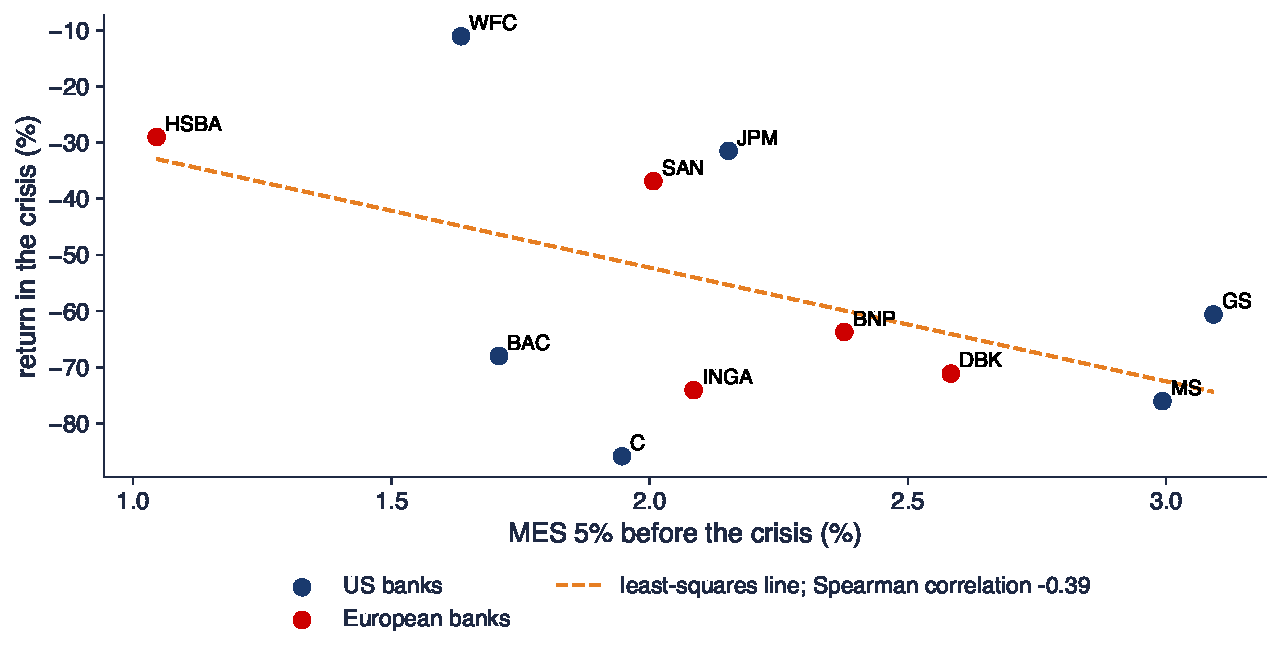
\includegraphics[width=0.97\textwidth,height=0.58\textheight,keepaspectratio]{sfm_ch15_mes_crisis.pdf}
\end{center}
\vspace{-0.25cm}
\begin{itemize}
    \item Designul din \refAPPR: MES 5\% măsurat din iunie 2006 pînă în iunie 2007, comparat cu randamentul din iulie 2007 pînă în decembrie 2008; aici 11 bănci americane și europene
    \item Corelația Spearman $-0{,}39$ (p $= 0{,}23$, $n = 11$): semnul din lucrare (MES mai mare, pierdere mai mare), dar nesemnificativ cu 11 bănci; cel mai prost randament: Citigroup ($-86\%$)
\end{itemize}
\sfmquantlet{Ch_15}{SFM_ch15_mes_srisk}
\end{frame}

\begin{frame}{De la MES la LRMES}
\itemsize{\small}
\begin{itemize}
    \item O criză durează luni: avem nevoie de pierderea băncii dacă piața scade cu 40\% în șase luni: \textbf{LRMES} (long-run MES, MES pe termen lung)
    \begin{itemize}
        \item aproximarea din \refAER: $\mathrm{LRMES} \approx 1 - \exp(-18 \times \mathrm{MES})$, cu MES pierderea zilnică (ca fracție) în zilele în care piața scade cu peste 2\%
    \end{itemize}
    \item Exemplu: MES $= 3\% = 0{,}03$: $\mathrm{LRMES} = 1 - e^{-0{,}54} = 1 - 0{,}583 = 41{,}7\%$
    \begin{itemize}
        \item banca ar pierde aproximativ 41{,}7\% din valoarea de piață într-o astfel de criză
    \end{itemize}
    \item Cele 13 bănci: LRMES între 40\% și 65\%; Brownlees și Engle îl estimează în schimb dintr-un model dinamic (GARCH și corelație dinamică) \refBE
\end{itemize}
\end{frame}

\begin{frame}{SRISK: deficitul de capital într-o criză}
\itemsize{\small}
\begin{itemize}
    \item O bancă are nevoie de capital propriu de cel puțin o fracție $k$ din active; $k = 8\%$ în \refBE
    \begin{itemize}
        \item $D$: valoarea contabilă a datoriilor; $W$: valoarea de piață a capitalului propriu; activele $\approx D + W$
    \end{itemize}
    \item \textbf{SRISK} $= k(D + W_{\text{criză}}) - W_{\text{criză}}$ cu $W_{\text{criză}} = (1 - \mathrm{LRMES})W$:
    \begin{itemize}
        \item $\mathrm{SRISK} = kD - (1 - k)(1 - \mathrm{LRMES})\,W$ \refBE
        \item SRISK $> 0$: capital lipsă într-o criză; \textbf{SRISK agregat} (suma valorilor pozitive) este ceea ce statul ar putea fi nevoit să acopere
    \end{itemize}
    \item Exemplu: $D = 900$, $W = 100$ (miliarde), LRMES $= 41{,}7\%$
    \begin{itemize}
        \item SRISK $= 0{,}08 \times 900 - 0{,}92 \times (1 - 41{,}7\%) \times 100 = 72 - 53{,}6 = 18{,}4$ miliarde
    \end{itemize}
\end{itemize}
\end{frame}

\begin{frame}{SRISK și efectul de levier}
\itemsize{\footnotesize}
\begin{center}
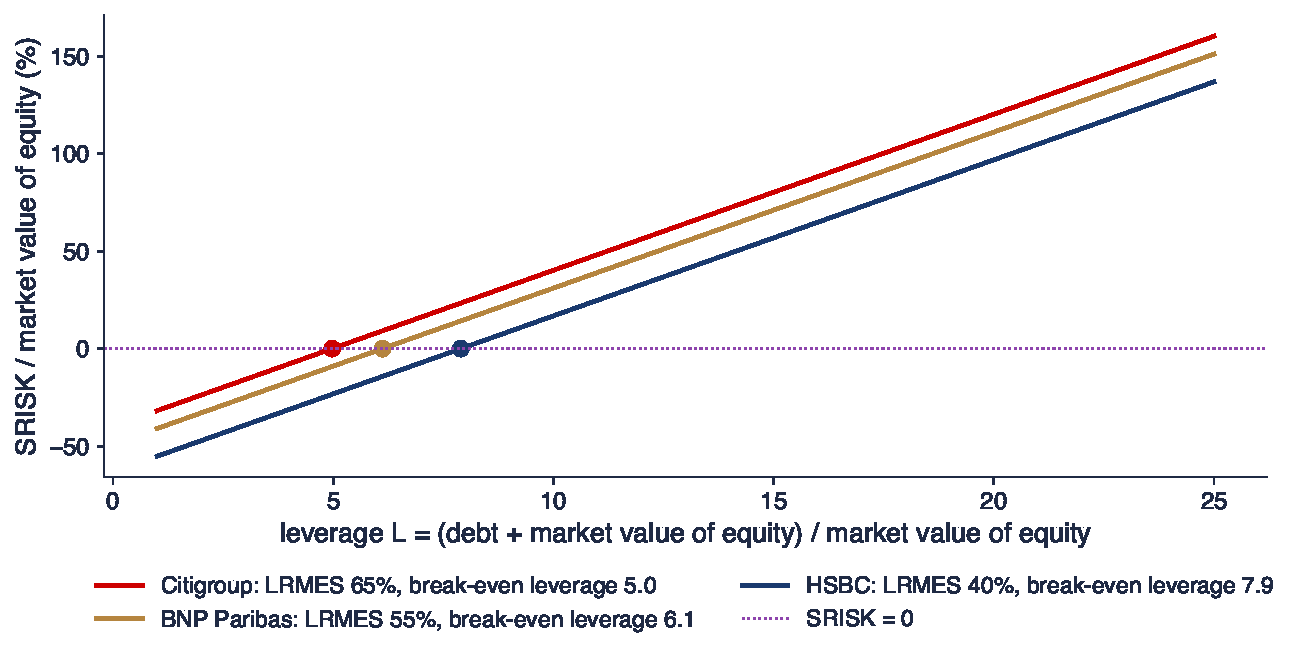
\includegraphics[width=0.97\textwidth,height=0.58\textheight,keepaspectratio]{sfm_ch15_srisk.pdf}
\end{center}
\vspace{-0.25cm}
\begin{itemize}
    \item SRISK$/W = k(L - 1) - (1 - k)(1 - \mathrm{LRMES})$, cu efectul de levier $L = (D + W)/W$; SRISK $> 0$ peste $L^* = 1 + (1 - k)(1 - \mathrm{LRMES})/k$
    \item Interpretare: Citigroup are nevoie de capital într-o criză peste un efect de levier de 5{,}0, HSBC doar peste 7{,}9; băncile au de regulă $L$ între 10 și 20, deci efectul de levier decide semnul
\end{itemize}
\sfmquantlet{Ch_15}{SFM_ch15_mes_srisk}
\end{frame}

\begin{frame}{Studiu de caz: SRISK și V-Lab}
\itemsize{\footnotesize}
\begin{columns}[T]
\begin{column}{0.56\textwidth}
\begin{itemize}
    \item \refBE: SRISK pentru marile firme financiare americane, cu LRMES dintr-un model GARCH--DCC (\sfmchlink{https://danpele.github.io/SFM/RO/Cursuri/capitol9_modele_arch_garch.pdf}{Capitolul 9})
    \begin{itemize}
        \item SRISK agregat a crescut înainte de falimentul Lehman; ajută la prognoza scăderilor producției industriale și a creșterii șomajului
        \item ordonarea după SRISK din 2007--2008 indică instituțiile care au avut ulterior nevoie de sprijin public
    \end{itemize}
    \item Europa: \refEJR; se folosește un $k = 5{,}5\%$ mai mic din cauza regulilor contabile (IFRS, International Financial Reporting Standards)
    \begin{itemize}
        \item publicat și actualizat pe \refVLab{} (NYU Stern) pentru instituții financiare din multe țări
    \end{itemize}
\end{itemize}
\end{column}
\begin{column}{0.42\textwidth}
\begin{columns}[T]
\begin{column}{0.48\textwidth}
\centering

\includegraphics[height=0.30\textheight]{ch15_acharya_2014.jpg}\\[1mm]
\imgcap{Viral Acharya}
\imgcredit{https://commons.wikimedia.org/wiki/File:Viral_Acharya_(2014).jpg}{Foto: MeJudice (2014); CC BY 3.0; Wikimedia Commons}
\end{column}
\begin{column}{0.48\textwidth}
\centering

\includegraphics[height=0.30\textheight]{ch9_engle_2022.jpg}\\[1mm]
\imgcap{Robert Engle}
\imgcredit{https://commons.wikimedia.org/wiki/File:0603-Kraneshares_KRBN-RobertEngle-JonDemske-16_(cropped).jpg}{Foto: Jon Demske (2022); CC BY-SA 4.0; Wikimedia Commons}
\end{column}
\end{columns}
\end{column}
\end{columns}
\end{frame}

\begin{frame}{Recapitulare: MES și SRISK}
\itemsize{\small}
\begin{itemize}
    \item MES 5\%: pierderea medie a unei bănci în cele mai proaste 5\% dintre zilele pieței; LRMES $\approx 1 - \exp(-18\,\mathrm{MES})$
    \item SRISK $= kD - (1 - k)(1 - \mathrm{LRMES})W$: capitalul lipsă într-o criză, determinat de efectul de levier și de LRMES
    \item MES, $\Delta$CoVaR și VaR răspund la întrebări diferite și ordonează diferit băncile
\end{itemize}
\end{frame}


%=============================================================================
\section{Rețele de bănci}
%=============================================================================

\begin{frame}{Perspectiva rețelei}
\itemsize{\small}
\begin{itemize}
    \item O \textbf{rețea}: noduri (bănci) și legături orientate („un șoc la $i$ îl afectează pe $j$”)
    \begin{itemize}
        \item legăturile reale (creditele interbancare) sînt în mare parte confidențiale; estimăm legăturile din randamente
    \end{itemize}
    \item Două instrumente statistice
    \begin{itemize}
        \item \textbf{Cauzalitatea Granger}: ajută randamentele trecute ale lui $i$ la prognoza lui $j$? \refBGLP
        \item \textbf{descompunerea varianței}: ce parte din eroarea de prognoză a lui $j$ vine din șocurile lui $i$? \refDYc
    \end{itemize}
    \item O legătură statistică este o mișcare comună, nu un contract: arată unde trebuie căutat, nu de ce
\end{itemize}
\end{frame}

\begin{frame}{Cauzalitatea Granger}
\itemsize{\small}
\begin{itemize}
    \item $x$ \textbf{cauzează în sens Granger} pe $y$ dacă valorile trecute ale lui $x$ îmbunătățesc prognoza lui $y$ dincolo de trecutul lui $y$ \refGranger
    \begin{itemize}
        \item regresia $y_t = a + b\,y_{t-1} + c\,x_{t-1} + e_t$; testăm $H_0: c = 0$ cu un test $t$ la 5\%
    \end{itemize}
    \item \textbf{Gradul de cauzalitate Granger} (DGC, degree of Granger causality) \refBGLP: proporția dintre cele $N(N-1)$ perechi ordonate cu o legătură semnificativă
    \begin{itemize}
        \item lucrarea: randamente lunare, ferestre mobile de 36 de luni, un decalaj, nivelul 5\%
        \item lucrarea filtrează în plus fiecare serie cu un model GARCH(1,1); cu 36 de observații lunare pe fereastră, raportăm testul nefiltrat
    \end{itemize}
    \item Fără legături, aproximativ 5\% dintre perechi sînt semnificative din întîmplare: DGC trebuie comparat cu 5\%
\end{itemize}
\end{frame}

\begin{frame}{Rețele Granger în timp}
\itemsize{\footnotesize}
\begin{center}
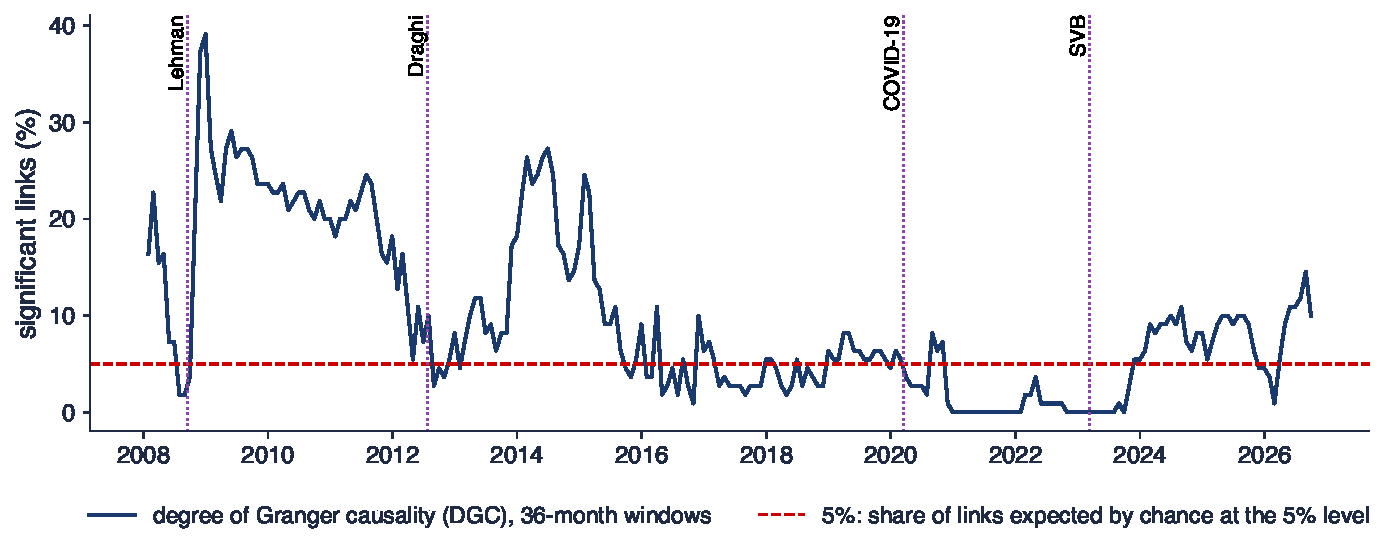
\includegraphics[width=0.97\textwidth,height=0.58\textheight,keepaspectratio]{sfm_ch15_dgc.pdf}
\end{center}
\vspace{-0.25cm}
\begin{itemize}
    \item 11 bănci americane și europene, randamente lunare din 2005 (260 de luni); prima fereastră se încheie în ianuarie 2008
    \item DGC: maximul 39\% (fereastra care se încheie pe 31 decembrie 2008), media 10\%, minimul 0\% (31 decembrie 2020)
\end{itemize}
\sfmquantlet{Ch_15}{SFM_ch15_networks}
\end{frame}

\begin{frame}{Două rețele: 2007--2009 și 2017--2019}
\itemsize{\footnotesize}
\begin{center}
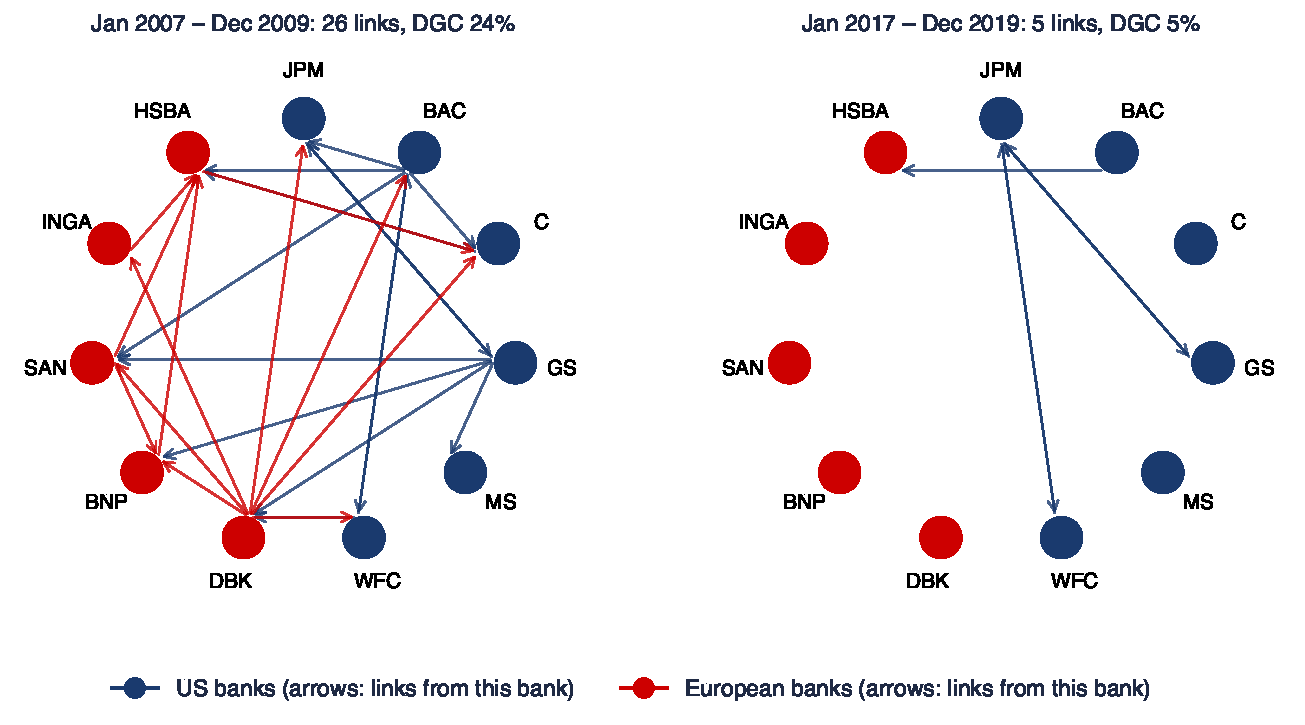
\includegraphics[width=0.97\textwidth,height=0.62\textheight,keepaspectratio]{sfm_ch15_granger_net.pdf}
\end{center}
\vspace{-0.25cm}
\begin{itemize}
    \item Săgeți: legăturile de cauzalitate Granger semnificative la 5\%, pe o fereastră de 36 de luni; numărul legăturilor: 26 în fereastra de criză, 5 în cea liniștită
    \item Interpretare: ca în \refBGLP, băncile au devenit mai conectate în jurul crizei; în anii liniștiți, rețeaua este apropiată de ceea ce ar da doar întîmplarea
\end{itemize}
\sfmquantlet{Ch_15}{SFM_ch15_networks}
\end{frame}

\begin{frame}{Conectivitatea Diebold--Yilmaz}
\itemsize{\small}
\begin{itemize}
    \item Estimăm un model VAR (vector autoregresiv) pe randamentele celor $N$ bănci; prognozăm pe $H$ zile
    \begin{itemize}
        \item $d_{ij}$: proporția din varianța erorii de prognoză pe $H$ zile a băncii $i$ datorată șocurilor băncii $j$ (descompunerea generalizată, \refPS)
        \item fiecare rînd însumează 100\%
    \end{itemize}
    \item Măsuri \refDYb; \refDYc
    \begin{itemize}
        \item FROM (de la celelalte): $\sum_{j \ne i} d_{ij}$; TO (către celelalte): $\sum_{j \ne i} d_{ji}$; NET $=$ TO $-$ FROM
        \item \textbf{conectivitatea totală}: $\frac{1}{N}\sum_{i \ne j} d_{ij}$, proporția medie a riscului care vine de la celelalte bănci
    \end{itemize}
    \item Aici: randamentele zilnice ale celor 11 bănci din 2005, ordinul VAR ales prin BIC (Bayesian information criterion, criteriul informațional Bayesian), $H = 10$ zile
\end{itemize}
\end{frame}

\begin{frame}{Tabelul de conectivitate}
\itemsize{\footnotesize}
\begin{center}
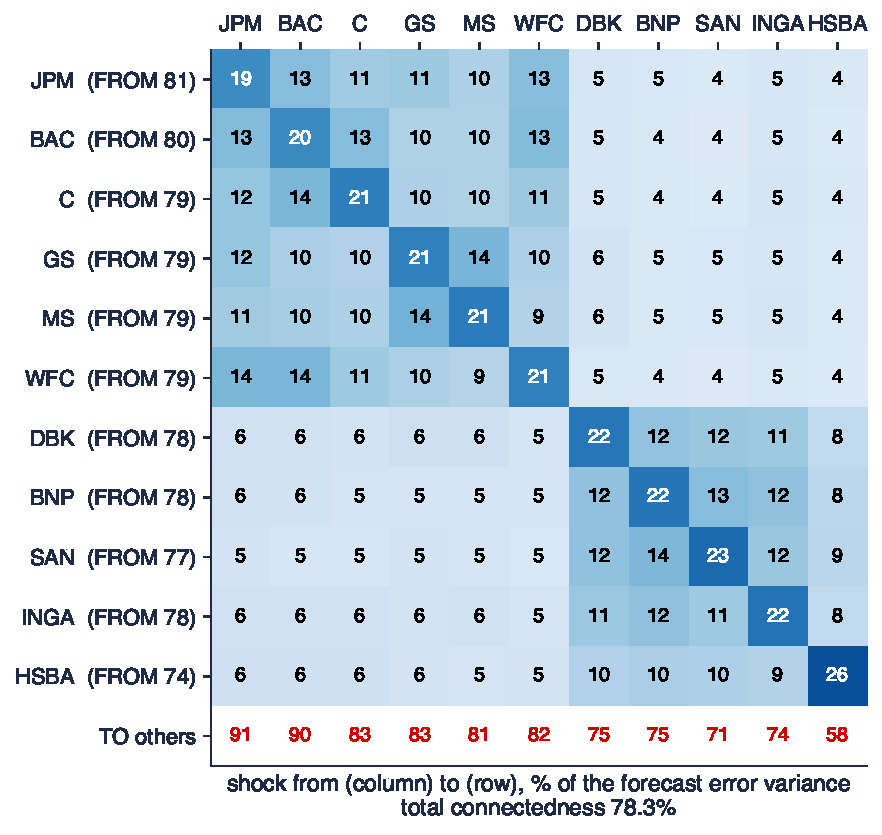
\includegraphics[width=0.97\textwidth,height=0.64\textheight,keepaspectratio]{sfm_ch15_dy_table.pdf}
\end{center}
\vspace{-0.25cm}
\begin{itemize}
    \item 4\,895 de zile comune, VAR(1); conectivitatea totală 78{,}3\%; două blocuri: băncile americane sînt conectate mai ales între ele, cele europene la fel
    \item Cel mai mare transmițător (TO): JPMorgan Chase; cel mai mic: HSBC (NET $-15{,}8$)
\end{itemize}
\sfmquantlet{Ch_15}{SFM_ch15_networks}
\end{frame}

\begin{frame}{Interpretarea tabelului de conectivitate}
\itemsize{\small}
\begin{itemize}
    \item Fiecare bancă primește aproximativ patru cincimi din varianța erorii de prognoză de la celelalte (FROM între 74 și 81)
    \begin{itemize}
        \item randamentele zilnice ale băncilor sînt dominate de șocuri comune; partea proprie (diagonala) este doar de aproximativ o cincime
    \end{itemize}
    \item NET: băncile americane sînt transmițători neți (JPMorgan Chase $+10{,}6$), cele europene receptori neți (HSBC $-15{,}8$)
    \begin{itemize}
        \item parțial din cauza orelor: New York închide după Europa, deci știrile americane ajung în prețurile europene a doua zi
    \end{itemize}
    \item Conectivitatea descrie datele; nu este o hartă a expunerilor dintre bănci
\end{itemize}
\end{frame}

\begin{frame}{Conectivitatea totală în timp}
\itemsize{\footnotesize}
\begin{center}
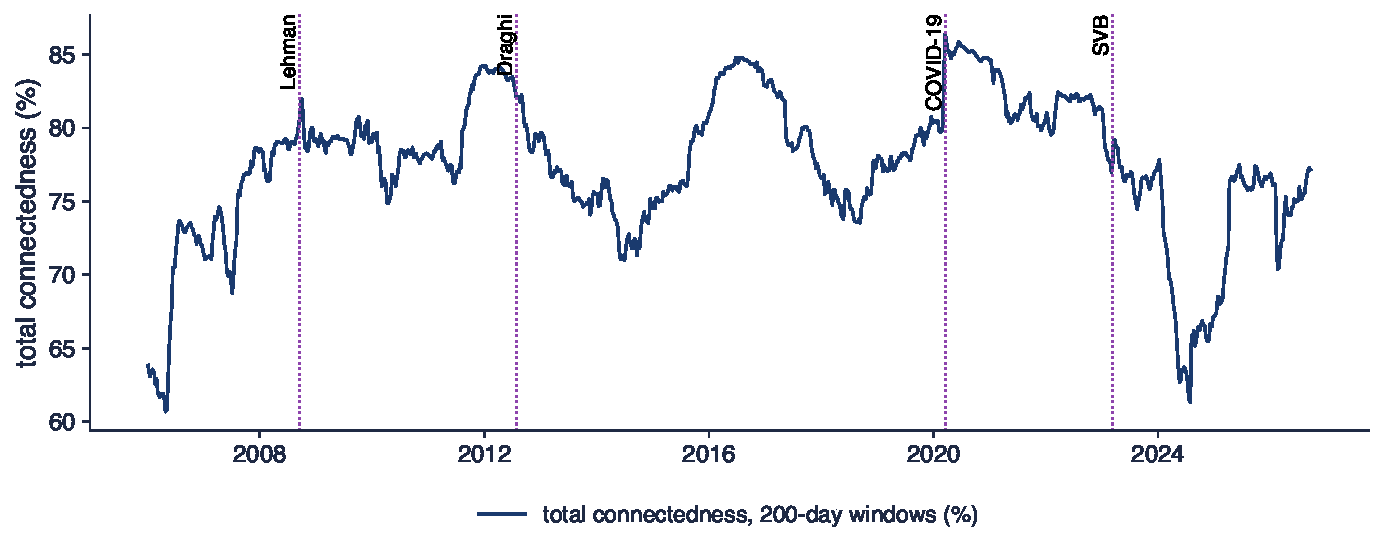
\includegraphics[width=0.97\textwidth,height=0.58\textheight,keepaspectratio]{sfm_ch15_dy_rolling.pdf}
\end{center}
\vspace{-0.25cm}
\begin{itemize}
    \item Ferestre mobile de 200 de zile, deplasate cu 5 zile; minimul 61\% (28 aprilie 2006), maximul 86\% (17 martie 2020); octombrie 2008 -- martie 2009: 79\%
    \item Interpretare: conectivitatea a crescut în 2007, înainte de Lehman, și atinge maximele în crize; scade cînd domină știrile specifice fiecărei bănci (2006, 2024)
\end{itemize}
\sfmquantlet{Ch_15}{SFM_ch15_networks}
\end{frame}

\begin{frame}{Lectură suplimentară: Financial Risk Meter}
\itemsize{\small}
\begin{itemize}
    \item \textbf{FRM} (Financial Risk Meter, indicatorul riscului financiar) \refFRM: un indice zilnic al riscului sistemic, din regresii cuantilice cu mulți regresori
    \begin{itemize}
        \item pentru fiecare bancă: o regresie cuantilică lasso (\sfmchlink{https://danpele.github.io/SFM/RO/Cursuri/capitol13_invatare_automata.pdf}{Capitolul 13}) a randamentelor sale pe randamentele tuturor celorlalte bănci și pe variabile macroeconomice
        \item penalizarea $\lambda$ necesară pentru a ajusta coada este mare cînd băncile se mișcă împreună: FRM = media valorilor $\lambda$
    \end{itemize}
    \item Extinderi
    \begin{itemize}
        \item TENET (tail-event driven network, rețea condusă de evenimentele din coadă) \refTENET: CoVaR cu multe bănci, o rețea de legături în coadă
        \item FRM pentru piețele emergente \refFRMem; cursul video de pe Quantinar (Bibliografie și instrumente)
    \end{itemize}
\end{itemize}
\end{frame}

\begin{frame}{Recapitulare: rețele}
\itemsize{\small}
\begin{itemize}
    \item Rețelele Granger: proporția legăturilor semnificative (DGC) comparată cu 5\%, cît dă întîmplarea; a crescut în jurul anului 2008
    \item Diebold--Yilmaz: proporții din varianța erorii de prognoză; TO, FROM, NET și indicele total
    \item Legăturile statistice arată mișcarea comună din date; nu dezvăluie contractele din spatele ei
\end{itemize}
\end{frame}


%=============================================================================
\section{Politica macroprudențială}
%=============================================================================

\begin{frame}{Microprudențial și macroprudențial}
\itemsize{\small}
\begin{itemize}
    \item \textbf{Microprudențial}: este fiecare bancă sigură luată separat? (capital, VaR, backtesting, \sfmchlink{https://danpele.github.io/SFM/RO/Cursuri/capitol10_var_es_backtesting.pdf}{Capitolul 10})
    \item \textbf{Macroprudențial}: este sistemul sigur? Două dimensiuni
    \begin{itemize}
        \item \textbf{în timp}: riscul se acumulează în perioadele de avînt (creditare, efect de levier) și devine vizibil în crize: se constituie amortizoare în perioadele bune
        \item \textbf{între instituții}: băncile mai mari și mai interconectate au nevoie de mai mult capital
    \end{itemize}
    \item Măsurile din acest capitol (CoVaR, SRISK, conectivitatea) se numără printre instrumentele cu care băncile centrale urmăresc a doua dimensiune
\end{itemize}
\end{frame}

\begin{frame}{Amortizoarele de capital din Basel III}
\itemsize{\footnotesize}
\begin{columns}[T]
\begin{column}{0.62\textwidth}
\begin{itemize}
    \item Capitalul CET1 (common equity tier 1, capital comun de nivel 1) minim: 4,5\% din activele ponderate la risc \refBIII; peste el, amortizoare \refRBC:
    \begin{itemize}
        \item \textbf{amortizorul de conservare a capitalului}: 2,5\%; sub el, dividendele și bonusurile sînt restricționate
        \item \textbf{amortizorul anticiclic}: 0--2,5\%, crescut cînd creditul crește prea repede și eliberat într-o criză
    \end{itemize}
    \item Pentru importanța sistemică
    \begin{itemize}
        \item \textbf{suplimentul G-SIB}: între 1\% și 3,5\%, după un scor al mărimii, interconectării, substituibilității, complexității și activității transfrontaliere \refGSIB
        \item în UE: amortizoare O-SII (other systemically important institutions, alte instituții de importanță sistemică) și un amortizor pentru riscul sistemic
    \end{itemize}
\end{itemize}
\end{column}
\begin{column}{0.34\textwidth}
\centering
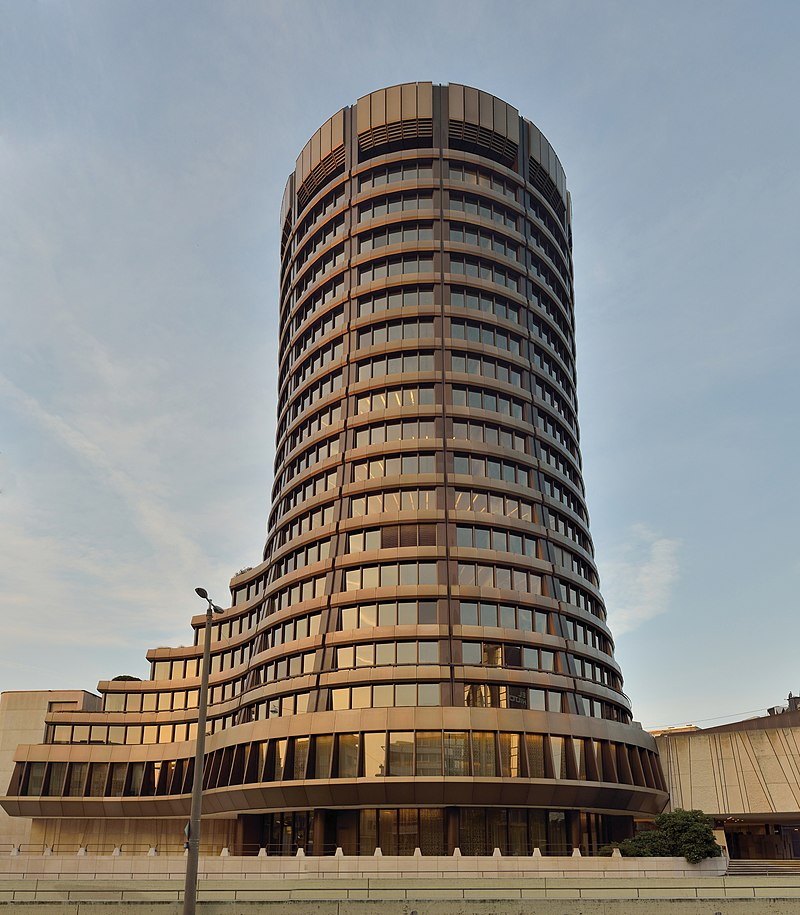
\includegraphics[height=0.36\textheight]{ch10_bis_tower_2014.jpg}\\[1mm]
\imgcap{Turnul BIS din Basel}
\imgcredit{https://commons.wikimedia.org/wiki/File:Basel_Committee_on_Banking_Supervision_-_BCBS.jpg}{Foto: Taxiarchos228 (2014); CC BY-SA 4.0; Wikimedia Commons}
\end{column}
\end{columns}
\end{frame}

\begin{frame}{Cine aplică politica: ESRB și BNR}
\itemsize{\footnotesize}
\begin{columns}[T]
\begin{column}{0.60\textwidth}
\begin{itemize}
    \item \textbf{ESRB} (European Systemic Risk Board, Comitetul European pentru Risc Sistemic), înființat în 2010, după criză, condus de președintele ECB \refESRB
    \begin{itemize}
        \item urmărește riscul sistemic în UE și emite avertismente și recomandări către autoritățile naționale
    \end{itemize}
    \item România: \textbf{CNSM} (Comitetul Național pentru Supravegherea Macroprudențială), cu BNR, ASF (Autoritatea de Supraveghere Financiară) și Guvernul \refCNSM
    \begin{itemize}
        \item BNR stabilește amortizoarele de capital ale băncilor (anticiclic, O-SII, pentru riscul sistemic) pe baza recomandărilor CNSM
        \item BNR folosește și limite pentru debitori (gradul de îndatorare, raportul dintre credit și valoarea garanției) și publică un raport asupra stabilității financiare
    \end{itemize}
\end{itemize}
\end{column}
\begin{column}{0.36\textwidth}
\centering
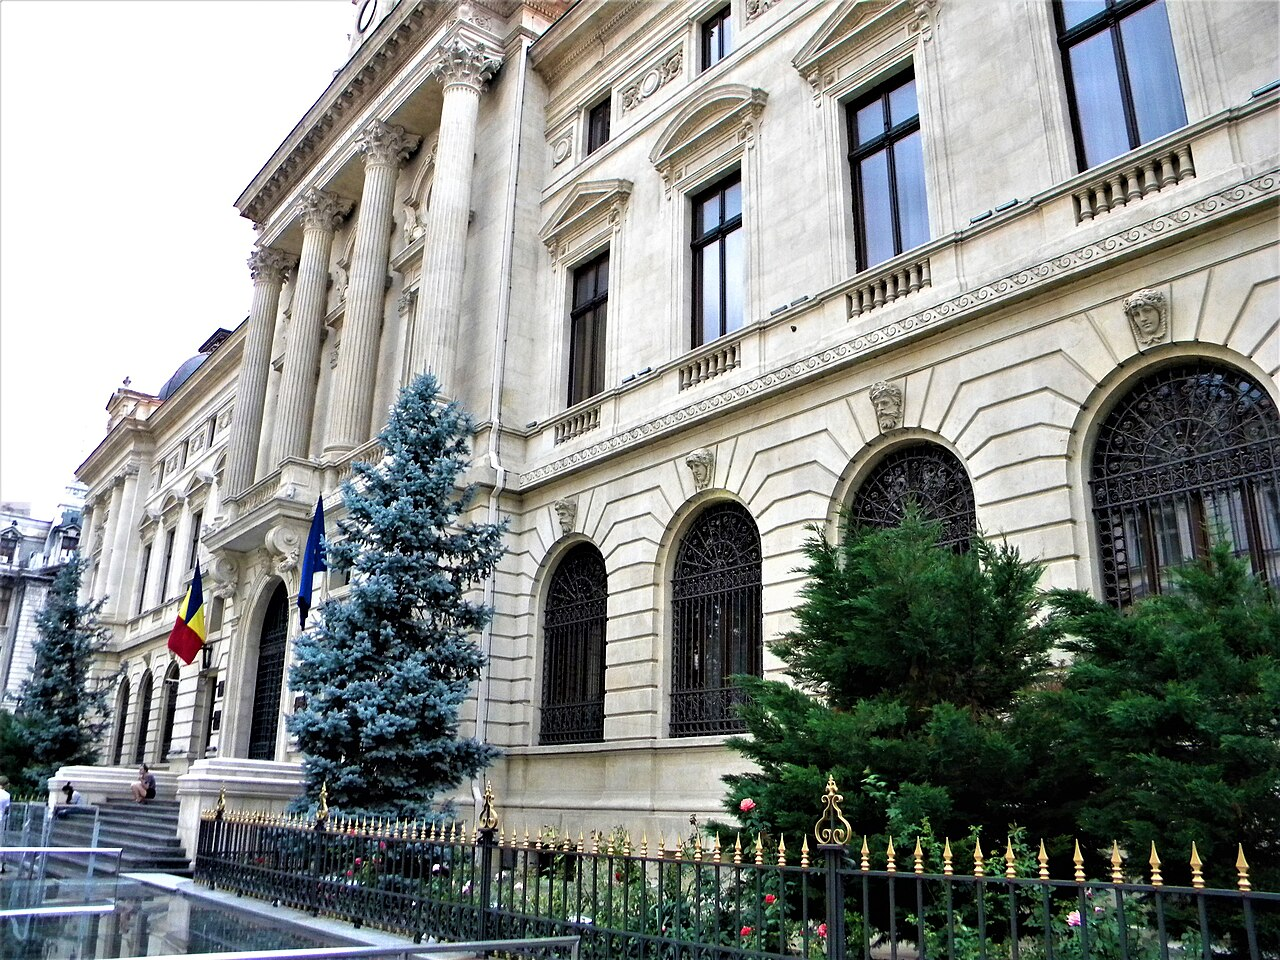
\includegraphics[height=0.36\textheight]{ch15_bnr_palace_2018.jpg}\\[1mm]
\imgcap{Palatul BNR din București}
\imgcredit{https://commons.wikimedia.org/wiki/File:Bucuresti,_Romania._BANCA_NATIONALA_A_ROMANIEI_(2)_(B-II-m-A-19023).jpg}{Foto: Britchi Mirela (2018); CC BY-SA 4.0; Wikimedia Commons}
\end{column}
\end{columns}
\end{frame}

\begin{frame}{Recapitulare: politica macroprudențială}
\itemsize{\small}
\begin{itemize}
    \item Politica macroprudențială vizează sistemul: amortizoare constituite în perioadele bune, capital suplimentar pentru băncile sistemice
    \item Basel III: 4,5\% CET1 + 2,5\% conservare + 0--2,5\% anticiclic + suplimente G-SIB / O-SII
    \item UE: ESRB; România: CNSM, cu BNR aplicînd amortizoarele de capital
\end{itemize}
\end{frame}


%=============================================================================
\section{AI pentru descoperire științifică}
%=============================================================================

\begin{frame}{O întrebare deschisă}
\itemsize{\small}
\begin{itemize}
    \item \textbf{Este riscul sistemic al băncilor românești importat de la băncile-mamă din zona euro sau este local?}
    \begin{itemize}
        \item azi: $\Delta$CoVaR al TLV atinge maximul în martie 2020 ($12{,}81\%$); BRD aparține unui grup francez, TLV are acționariat românesc
        \item BET este parțial chiar băncile, deci este nevoie de un „sistem” mai bun
    \end{itemize}
    \item Întrebarea rămîne deschisă: două bănci, puține crize, ore de tranzacționare diferite (București, Frankfurt, New York), lichiditate redusă în unii ani
    \item Instrumentele AI pot accelera un astfel de studiu; nu înlocuiesc verificarea lui \refWang
\end{itemize}
\end{frame}

\begin{frame}{Contribuția posibilă a AI}
\itemsize{\small}
\begin{itemize}
    \item \textbf{Literatura}: o listă a studiilor despre riscul sistemic în Europa Centrală și de Est și despre contagiunea dintre băncile-mamă și filiale
    \item \textbf{Cod}: o primă versiune a $\Delta$CoVaR pentru TLV și BRD, cu portofoliul băncilor din zona euro ca variabilă de condiționare și cu variabile de stare
    \item \textbf{Robustețe}: randamente pe două zile (orele de tranzacționare), date săptămînale, CoVaR la 5\%, alte variabile de stare
    \item Exemplu de prompt
    \begin{itemize}
        \item \aiprompt{Write Python code that estimates the Delta-CoVaR at 1\% of the BET conditional on Banca Transilvania by quantile regression, with the lagged VIX and the lagged Euro Stoxx 50 return as state variables, and adds a moving-block bootstrap interval.}
    \end{itemize}
\end{itemize}
\end{frame}

\begin{frame}{Verificări necesare}
\itemsize{\small}
\begin{itemize}
    \item Convenția nivelului: „CoVaR 1\%” și „MES 5\%” indică probabilitatea cozii; CoVaR și MES sînt pierderi pozitive
    \item Direcția condiționării: CoVaR este sistemul condiționat de bancă, MES este banca condiționată de piață
    \item $\Delta$CoVaR compară situația de criză cu \textbf{mediana} băncii, nu cu VaR-ul băncii
    \item Prețurile se aliniază pe zilele comune înainte de calculul randamentelor; zilele BVB fără tranzacții se elimină; orele de tranzacționare diferă
    \item Incertitudinea: regresiile cuantilice la 1\% se sprijină pe aproximativ 1\% dintre zile; raportați intervale bootstrap
    \item Referințele: fiecare lucrare citată trebuie să existe; verificați DOI-ul
\end{itemize}
\end{frame}

\begin{frame}{Idee de proiect}
\itemsize{\small}
\begin{itemize}
    \item \textbf{Întrebarea}: cresc băncile din zona euro riscul din coadă al băncilor românești în perioadele de stres?
    \begin{itemize}
        \item date: TLV, BRD, BET, cele cinci bănci europene, Euro Stoxx 50, VIX, din 2010 (EODHD)
    \end{itemize}
    \item Pași
    \begin{itemize}
        \item $\Delta$CoVaR 1\% al fiecărei bănci românești condiționat de portofoliul băncilor europene, static și cu variabile de stare
        \item MES 5\% pentru TLV și BRD, cu Euro Stoxx 50 ca piață; proporțiile FROM Diebold--Yilmaz pe ferestre mobile
        \item comparați 2011--2012, martie 2020 și martie 2023, cu intervale bootstrap pe blocuri
    \end{itemize}
    \item Livrabil: un tabel, un grafic și un paragraf despre ce pot și ce nu pot arăta datele
    \item Declarați orice utilizare a instrumentelor AI și enumerați erorile acestora pe care le-ați corectat
\end{itemize}
\end{frame}


%=============================================================================
\section{Rezumat}
%=============================================================================

\begin{frame}{Idei de reținut}
\itemsize{\small}
\begin{itemize}
    \item Riscul sistemic este o proprietate a sistemului: contagiune, expuneri comune, vînzări forțate și retrageri masive, amplificate de efectul de levier
    \item În crize, corelațiile și dependența în cozi dintre bănci cresc; corectați pentru volatilitate înainte de a vorbi despre contagiune
    \item CoVaR 1\%: sistemul condiționat de bancă; $\Delta$CoVaR $= \hat b(\hat q_{50\%} - \hat q_\alpha)$ din regresia cuantilică
    \item MES 5\%: banca condiționată de piață; SRISK $= kD - (1 - k)(1 - \mathrm{LRMES})W$, determinat de efectul de levier
    \item Rețelele (Granger, Diebold--Yilmaz) arată o conectivitate mai mare în jurul crizelor
    \item Politica macroprudențială: amortizoarele Basel III, suplimentele G-SIB și O-SII; ESRB în UE, CNSM și BNR în România
\end{itemize}
\end{frame}

\begin{frame}{Formule de reținut}
\itemsize{\small}
{\renewcommand{\arraystretch}{1.45}\begin{center}
\scriptsize
\begin{tabular}{ll}
\toprule
\textbf{Mărimea} & \textbf{Formula} \\
\midrule
CoVaR & $\mathrm{CoVaR}_\alpha = -(\hat a + \hat b\,\hat q_\alpha(X^i))$, \ $X^{sys} = a + bX^i$ la nivelul $\alpha$ \\
$\Delta$CoVaR & $\hat b\,(\hat q_{50\%}(X^i) - \hat q_\alpha(X^i))$ \\
MES & $-E[X^i \mid X^m \le q_\alpha(X^m)]$ \\
LRMES & $1 - \exp(-18\,\mathrm{MES}_{2\%})$ \\
SRISK & $kD - (1 - k)(1 - \mathrm{LRMES})W$, \ $L^* = 1 + (1 - k)(1 - \mathrm{LRMES})/k$ \\
Forbes--Rigobon & $\rho^* = \rho/\sqrt{1 + \delta(1 - \rho^2)}$ \\
Granger & $y_t = a + by_{t-1} + cx_{t-1} + e_t$, \ $H_0: c = 0$ \\
Diebold--Yilmaz & total $= \frac1N\sum_{i \ne j} d_{ij}$, \ NET$_i = $ TO$_i - $ FROM$_i$ \\
\bottomrule
\end{tabular}
\end{center}
}
\end{frame}

\begin{frame}{Autoevaluare}
\itemsize{\small}
\begin{itemize}
    \item \textbf{Întrebare}: banca A are un VaR 1\% mai mare decît banca B. Este A mai importantă sistemic?
    \begin{itemize}
        \item \textbf{Răspuns}: nu neapărat: importanța sistemică depinde de legătura cu sistemul ($\Delta$CoVaR, MES), nu de coada proprie a băncii
    \end{itemize}
    \item \textbf{Întrebare}: o regresie cuantilică la 1\% dă $\hat b = 0{,}5$, $\hat q_{1\%}(X^i) = -6\%$, $\hat q_{50\%}(X^i) = 0$. Cît este $\Delta$CoVaR?
    \begin{itemize}
        \item \textbf{Răspuns}: $0{,}5 \times (0 - (-6)) = 3\%$
    \end{itemize}
    \item \textbf{Întrebare}: de ce poate fi SRISK negativ?
    \begin{itemize}
        \item \textbf{Răspuns}: o bancă cu efect de levier mic rămîne cu suficient capital chiar și după o scădere a pieței de 40\%: are un surplus de capital
    \end{itemize}
    \item Urmează: \sfmchlink{https://danpele.github.io/SFM/RO/Cursuri/capitol16_recapitulare.pdf}{Capitolul 16}, recapitulare
\end{itemize}
\end{frame}


%=============================================================================
\section{Bibliografie}
%=============================================================================

\begin{frame}{Bibliografie (1/3)}
\itemsize{\tiny}
\begin{itemize}
    \item Acharya, V.V., Engle, R., Richardson, M. (2012). \href{https://doi.org/10.1257/aer.102.3.59}{Capital shortfall: a new approach to ranking and regulating systemic risks}. \textit{American Economic Review}, 102(3), 59--64.
    \item Acharya, V.V., Pedersen, L.H., Philippon, T., Richardson, M. (2017). \href{https://doi.org/10.1093/rfs/hhw088}{Measuring systemic risk}. \textit{Review of Financial Studies}, 30(1), 2--47.
    \item Adrian, T., Brunnermeier, M.K. (2016). \href{https://doi.org/10.1257/aer.20120555}{CoVaR}. \textit{American Economic Review}, 106(7), 1705--1741.
    \item Allen, F., Gale, D. (2000). \href{https://doi.org/10.1086/262109}{Financial contagion}. \textit{Journal of Political Economy}, 108(1), 1--33.
    \item Basel Committee on Banking Supervision (2011). \href{https://www.bis.org/publ/bcbs189.htm}{Basel III: a global regulatory framework for more resilient banks and banking systems}, revised June 2011. Bank for International Settlements.
    \item Basel Committee on Banking Supervision (2018). \href{https://www.bis.org/bcbs/publ/d445.htm}{Global systemically important banks: revised assessment methodology and the higher loss absorbency requirement}. Bank for International Settlements.
    \item Ben Amor, S., Althof, M., Härdle, W.K. (2022). \href{https://doi.org/10.1016/j.ribaf.2021.101594}{Financial Risk Meter for emerging markets}. \textit{Research in International Business and Finance}, 60, 101594.
    \item Benoit, S., Colliard, J.-E., Hurlin, C., Pérignon, C. (2017). \href{https://doi.org/10.1093/rof/rfw026}{Where the risks lie: a survey on systemic risk}. \textit{Review of Finance}, 21(1), 109--152.
    \item Billio, M., Getmansky, M., Lo, A.W., Pelizzon, L. (2012). \href{https://doi.org/10.1016/j.jfineco.2011.12.010}{Econometric measures of connectedness and systemic risk in the finance and insurance sectors}. \textit{Journal of Financial Economics}, 104(3), 535--559.
    \item Bisias, D., Flood, M., Lo, A.W., Valavanis, S. (2012). \href{https://doi.org/10.1146/annurev-financial-110311-101754}{A survey of systemic risk analytics}. \textit{Annual Review of Financial Economics}, 4, 255--296.
    \item Brownlees, C., Engle, R.F. (2017). \href{https://doi.org/10.1093/rfs/hhw060}{SRISK: a conditional capital shortfall measure of systemic risk}. \textit{Review of Financial Studies}, 30(1), 48--79.
    \item Brunnermeier, M.K., Pedersen, L.H. (2009). \href{https://doi.org/10.1093/rfs/hhn098}{Market liquidity and funding liquidity}. \textit{Review of Financial Studies}, 22(6), 2201--2238.
    \item Demarta, S., McNeil, A.J. (2005). \href{https://doi.org/10.1111/j.1751-5823.2005.tb00254.x}{The t copula and related copulas}. \textit{International Statistical Review}, 73(1), 111--129.
    \item Diamond, D.W., Dybvig, P.H. (1983). \href{https://doi.org/10.1086/261155}{Bank runs, deposit insurance, and liquidity}. \textit{Journal of Political Economy}, 91(3), 401--419.
    \item Diebold, F.X., Yilmaz, K. (2009). \href{https://doi.org/10.1111/j.1468-0297.2008.02208.x}{Measuring financial asset return and volatility spillovers, with application to global equity markets}. \textit{Economic Journal}, 119(534), 158--171.
    \item Diebold, F.X., Yilmaz, K. (2012). \href{https://doi.org/10.1016/j.ijforecast.2011.02.006}{Better to give than to receive: predictive directional measurement of volatility spillovers}. \textit{International Journal of Forecasting}, 28(1), 57--66.
\end{itemize}
\end{frame}

\begin{frame}{Bibliografie (2/3)}
\itemsize{\tiny}
\begin{itemize}
    \item Diebold, F.X., Yilmaz, K. (2014). \href{https://doi.org/10.1016/j.jeconom.2014.04.012}{On the network topology of variance decompositions: measuring the connectedness of financial firms}. \textit{Journal of Econometrics}, 182(1), 119--134.
    \item Draghi, M. (2012). \href{https://www.ecb.europa.eu/press/key/date/2012/html/sp120726.en.html}{Speech at the Global Investment Conference}, London, 26 July 2012. European Central Bank.
    \item Engle, R., Jondeau, E., Rockinger, M. (2015). \href{https://doi.org/10.1093/rof/rfu012}{Systemic risk in Europe}. \textit{Review of Finance}, 19(1), 145--190.
    \item European Systemic Risk Board (2026). \href{https://www.esrb.europa.eu/about/background/html/index.en.html}{Background and tasks}. Frankfurt am Main.
    \item Federal Deposit Insurance Corporation (2023). \href{https://www.fdic.gov/resources/resolutions/bank-failures/failed-bank-list/silicon-valley.html}{Silicon Valley Bank, Santa Clara, CA}. Failed bank information.
    \item Federal Reserve Board (2023). \href{https://www.federalreserve.gov/publications/files/svb-review-20230428.pdf}{Review of the Federal Reserve's supervision and regulation of Silicon Valley Bank}. Washington, DC, April 2023.
    \item FINMA (2023). \href{https://www.finma.ch/en/news/2023/03/20230319-mm-cs-ubs/}{FINMA approves merger of Credit Suisse and UBS}. Press release, 19 March 2023.
    \item Forbes, K.J., Rigobon, R. (2002). \href{https://doi.org/10.1111/0022-1082.00494}{No contagion, only interdependence: measuring stock market comovements}. \textit{Journal of Finance}, 57(5), 2223--2261.
    \item Franke, J., Härdle, W.K., Hafner, C.M. (2019). \href{https://doi.org/10.1007/978-3-030-13751-9}{\textit{Statistics of Financial Markets: An Introduction}}, 5th ed. Springer.
    \item Granger, C.W.J. (1969). \href{https://doi.org/10.2307/1912791}{Investigating causal relations by econometric models and cross-spectral methods}. \textit{Econometrica}, 37(3), 424--438.
    \item Haldane, A.G., May, R.M. (2011). \href{https://doi.org/10.1038/nature09659}{Systemic risk in banking ecosystems}. \textit{Nature}, 469, 351--355.
    \item Härdle, W.K., Wang, W., Yu, L. (2016). \href{https://doi.org/10.1016/j.jeconom.2016.02.013}{TENET: Tail-Event driven NETwork risk}. \textit{Journal of Econometrics}, 192(2), 499--513.
    \item IMF, BIS, FSB (2009). \href{https://www.bis.org/publ/othp07.htm}{Guidance to assess the systemic importance of financial institutions, markets and instruments: initial considerations}. Report to the G-20 Finance Ministers and Central Bank Governors.
    \item Koenker, R., Bassett, G. (1978). \href{https://doi.org/10.2307/1913643}{Regression quantiles}. \textit{Econometrica}, 46(1), 33--50.
    \item Mihoci, A., Althof, M., Chen, C.Y.-H., Härdle, W.K. (2020). \href{https://doi.org/10.1108/s0731-905320200000042016}{FRM Financial Risk Meter}. In \textit{The Econometrics of Networks}, Advances in Econometrics, 42, 335--368. Emerald.
    \item National Committee for Macroprudential Oversight (CNSM) (2026). \href{https://www.cnsmro.ro/}{Comitetul Național pentru Supravegherea Macroprudențială}. Bucharest.
\end{itemize}
\end{frame}

\begin{frame}{Bibliografie (3/3)}
\itemsize{\tiny}
\begin{itemize}
    \item Pesaran, H.H., Shin, Y. (1998). \href{https://doi.org/10.1016/S0165-1765(97)00214-0}{Generalized impulse response analysis in linear multivariate models}. \textit{Economics Letters}, 58(1), 17--29.
    \item Shleifer, A., Vishny, R. (2011). \href{https://doi.org/10.1257/jep.25.1.29}{Fire sales in finance and macroeconomics}. \textit{Journal of Economic Perspectives}, 25(1), 29--48.
    \item Wang, H., Fu, T., Du, Y., Gao, W., et al. (2023). \href{https://doi.org/10.1038/s41586-023-06221-2}{Scientific discovery in the age of artificial intelligence}. \textit{Nature}, 620, 47--60.
\end{itemize}
\end{frame}

\end{document}
